\documentclass[11pt,a4paper,oldfontcommands,oneside]{memoir}
\RequirePackage[english]{babel}
\usepackage[utf8]{inputenc}
\usepackage[T1]{fontenc}
\usepackage{microtype}
\usepackage{graphicx}
\usepackage{xcolor}
\usepackage{times}


\usepackage{url}
\usepackage{afterpage}
\usepackage{pstool}
\usepackage{comment}
\usepackage{wrapfig}
\usepackage[printonlyused]{acronym}
\usepackage{listings}
\usepackage{placeins}

\usepackage[
breaklinks=true,colorlinks=true,
linkcolor=blue,urlcolor=blue,citecolor=blue,% PDF VIEW
%linkcolor=black,urlcolor=black,citecolor=black,% PRINT
bookmarks=true,bookmarksopenlevel=2]{hyperref}

\usepackage{geometry}
% PDF VIEW
% \geometry{total={210mm,297mm},
% left=25mm,right=25mm,%
% bindingoffset=0mm, top=25mm,bottom=25mm}
% PRINT
\geometry{total={210mm,297mm},
left=20mm,right=20mm,
bindingoffset=10mm, top=25mm,bottom=25mm}


%\OnehalfSpacing
%\linespread{1.3}

%%% CHAPTER'S STYLE
\chapterstyle{bianchi}
%\chapterstyle{ger}
%\chapterstyle{madsen}
%\chapterstyle{ell}
%%% STYLE OF SECTIONS, SUBSECTIONS, AND SUBSUBSECTIONS
\setsecheadstyle{\Large\bfseries\sffamily\raggedright}
\setsubsecheadstyle{\large\bfseries\sffamily\raggedright}
\setsubsubsecheadstyle{\bfseries\sffamily\raggedright}


%%% STYLE OF PAGES NUMBERING
%\pagestyle{companion}\nouppercaseheads
%\pagestyle{headings}
%\pagestyle{Ruled}
\pagestyle{plain}
\makepagestyle{plain}
\makeevenfoot{plain}{\thepage}{}{}
\makeoddfoot{plain}{}{}{\thepage}
\makeevenhead{plain}{}{}{}
\makeoddhead{plain}{}{}{}

\setlength{\parindent}{0em}
\setlength{\parskip}{0.7em}

\maxsecnumdepth{subsection} % chapters, sections, and subsections are numbered
\maxtocdepth{subsection} % chapters, sections, and subsections are in the Table of Contents

\includeonly{c00,c01,c02,c03,c04,c05,c99}


\begin{document}

% -*- TeX -*- -*- UK -*- -*- Soft -*-
\chapter*{ABBREVIATIONS}
\addcontentsline{toc}{chapter}{ABBREVIATIONS}

% use:
%  \ac{IR}

\begin{acronym}\itemsep=-10pt\parsep=-10pt
\acro{2-D}{Two-Dimensional}
\acro{2D}{Two-Dimensional}
\acro{3-D}{Three-Dimensional}
\acro{3D}{Three-Dimensional}
\acro{A2D}{Analogue to Digital}
\acro{AAM}{Air-to-Air Missile}
\acro{AASRAM}{Air-to-Air Short Range Missile}
\acro{AA}{Air-to-Air}
\acro{ACE}{Adaptive Communication Environment}
\acro{AC}{Alternating Current}
\acro{ADC}{Analogue to Digital Converter}
\acro{AD}{Analogue to Digital (conversion)}
\acro{AFB}{Air Force Base}
\acro{AFCRL}{Air Force Cambridge Research Laboratories}
\acro{AFRL}{Air Force Research Laboratories}
\acro{AGC}{Automatic Gain Control}
\acro{AGL}{Above Ground Level}
\acro{AHP}{Analytical Hierarchy Process}
\acro{AI}{Artificial Intelligence}
\acro{AIM}{Air Intercept Missile}
\acro{AIRS}{Atmospheric Infrared Sounder}
\acro{AMBBB}{Ambient Temperature Blackbody}
\acro{AMRAAM}{Advanced Medium Range Air-to-Air Missile}
\acro{AM}{Amplitude Modulation}
\acro{ANSI}{American National Standards Institute}
\acro{API}{Application Programming Interface}
\acro{APU}{Auxiliary Power Unit}
\acro{ASCII}{American Standard Code for Information Interchange}
\acro{ASIC}{Application Specific Integrated Circuit}
\acro{ASL}{Above Sea Level}
\acro{ASRAAM}{Advanced Short Range Air-to-Air Missile}
\acro{ASU}{Air Support Unit}
\acro{ATP}{Acceptance Test Procedure}
\acro{ATR}{Automatic Target Recognition}
\acro{ATS}{Advanced Thermographic Systems}
\acro{AVI}{Audio Video Interleave}
\acro{BAe}{British Aerospace}
\acro{BB}{Black Body}
\acro{BCU}{Battery Coolant Unit}
\acro{BDI}{Buffered Direct Injection}
\acro{BDRF}{Bidirectional Reflection Function}
\acro{BFS}{Bomem File System}
\acro{BGRAMS}{Bomem Grams a software product}
\acro{BGT}{Bodenseewerk Ger\"atetechnik Gmbh}
\acro{BH}{I/O Bulkhead input/output}
\acro{BIT}{Built-in Test}
\acro{BLT}{Bilinear Transformation}
\acro{BNC}{Bayonet Neill-Concelman}
\acro{BPDF}{Bidirectional Polarization Distribution Functions}
\acro{BPR}{Bad Pixel Replacement}
\acro{BRDF}{Bidirectional Reflectance Distribution Function}
\acro{BSP}{Binary Space Partitions}
\acro{BVR}{Beyond Visual Range}
\acro{C$^4$I$^3$RS}{Command, Control, Communication, Computers, Information, Intelligence, Informatics, Reconnaissance and Surveillance}
\acro{CAD}{Computer Aided Design}
\acro{CAT}{Computed Axial Tomography}
\acro{CCD}{Charge Coupled Device}
\acro{CCIR}{Comite Consultatif International des Radio Communications}
\acro{CCM}{Counter-countermeasure}
\acro{CDSD}{Carbon Dioxide Spectroscopic Database}
\acro{CDS}{Correlated Double Sampling}
\acro{CD}{Compact Disk}
\acro{CEDIP}{Name of the camera manufacturer}
\acro{CFAR}{Constant False Alarm Rate}
\acro{CFI}{Customer Furnished Information}
\acro{CML}{Configurable Math Library}
\acro{CMOS}{Complementary Metal Oxide Semiconductor}
\acro{CmSim2}{Countermeasure Simulator (version 2)}
\acro{CmSim}{Countermeasure Simulator (version 1)}
\acro{CMS}{Classified MicroSeek}
\acro{CMT}{Cadmium Mercury Telluride}
\acro{CnC}{Command and Control}
\acro{CNES}{Centre National d'Etudes Spatiales, France}
\acro{CNR}{Clutter-to-noise ratio}
\acro{CNUC}{Continuous Non-Uniformity Correction}
\acro{CO$_2$}{Carbon Dioxide}
\acro{CODATA}{Committee on Data for Science and Technology}
\acro{COM}{Common Object Model}
\acro{CORBA}{Common Object Request Broker Architecture}
\acro{COTS}{Commercial of the Shelf}
\acro{CPU}{Central Processing Unit}
\acro{CSCI}{Computer Software Configuration Item}
\acro{CSIR}{Council for Scientific and Industrial Research}
\acro{CSV}{Comma Separated Variable}
\acro{CVS}{Concurrent Versions System}
\acro{CTAN}{Comprehensive TeX Archive Network}
\acro{CTIA} {Capacitive Transimpedance Amplifiers}
\acro{CVD}{Chemical vapour deposition}
\acro{DAS}{Denel Aerospace }
\acro{DCS}{Direct Current Subtraction}
\acro{DCM}{Direction Cosine Matrix}
\acro{DC}{Direct Current}
\acro{DD}{Denel Dynamics}
\acro{DEMS}{Digital Elevation Maps}
\acro{DEM}{Digital Elevation Map}
\acro{DFPN}{Dark current Fixed Pattern Noise}
\acro{DFT} {Discrete Fourier Transform}
\acro{DIRCM}{Directed Infrared Countermeasure}
\acro{DIRSIG}{Digital Imaging and Remote Sensing Image Generation}
\acro{DITSIM}{Directed Infrared Countermeasure and Imaging Toolkit Simulator}
\acro{DI}{Direct Injection}
\acro{DLE}{Differential Linearity Error }
\acro{DLSWC}{Denel Land Systems Western Cape}
\acro{DLU}{Directed Laser Unit}
\acro{DL}{Digital Level}
\acro{dl}{Digital Level}
\acro{DLea}[DL]{Deep Learning}
\acro{DLL}{Dynamic Load Library}
\acro{DOI}{Digital Object Identifier}
\acro{DOTR}{Denel Overberg Test Range}
\acro{DPA}{Digital Processing Assembly}
\acro{DPSS}{Defence, Peace Safety and Security, an operating unit of the CSIR}
\acro{DRI}{Detection, Recognition and Identification}
\acro{DSIM}{Directed Infrared Countermeasure Simulator}
\acro{DSP}{Digital Signal Processing}
\acro{DTD}{Document Type Definition}
\acro{DVD}{Digital Video Disk or Digital Versatile Disk}
\acro{ECCM}{Electronic Counter-Countermeasure}
\acro{ECEF}{Earth Centred Earth Fixed}
\acro{EDERI}{Electronic Defence Evaluation and Research Institute}
\acro{EDS}{Electronic Defence Systems}
\acro{EEPROM}{Electronically Erasable Programmable Read-Only Memory}
\acro{EGT}{Exhaust Gas Temperature}
\acro{EICAS}{Engine Indication and Crew Alert System}
\acro{EMF}{Electromotive force}
\acro{EMC}{Electromagnetic Compatibility}
\acro{EMI}{Electro-magnetic interference}
\acro{EMP}{Electro-magnetic pulse}
\acro{ENU}{East North Up}
\acro{ENVI}{An image processing product}
\acro{EofN}{east of north}
\acro{EOSS}{Electro-Optical Simulation System}
\acro{EO}{Electro Optics}
\acro{EPS}{European Polar System }
\acro{ESD}{East-South-Down (coordinate convention)}
\acro{EULA}{End-User Licence Agreement}
\acro{EUMETSAT}{EUropean organization for the exploitation of METeorological SATellites}
\acro{EWC}{Electronic Warfare Centre}
\acro{EW}{Electronic Warfare}
\acro{FAR}{False alarm rate}
\acro{FASCODE}{Fast Atmospheric Signature Code}
\acro{FET}{Field-Effect Transistor}
\acro{FIFO}{First In First Out memory system}
\acro{FIGHTERS}{ HITRAN Atmospheric Workstation}
\acro{FIRST}{Fourier Infrared Spectrometer Telops, an imaging FTIT camera}
\acro{FLIR}{Forward Looking Infrared (an infrared camera, also a company}
\acro{FMECA}{Failure modes, effects and criticality analysis}
\acro{FM}{Frequency Modulation}
\acro{FOM}{Figure of merit}
\acro{FOVEF}{Field of view Expansion Factor}
\acro{FOV}{Field of View}
\acro{FOR}{Field of Regard}
\acro{FPA}{Focal Plane Array}
\acro{FPGA}{Field-Programmable Gate Array}
\acro{FPN}{Fixed Pattern Noise}
\acro{FPO}{Fixed Pattern Offset}
\acro{FPP}{Focal Plane Processor}
\acro{FR}{Frame Rate}
\acro{FTIR}{Fourier-transform infrared spectrometer}
\acro{FTSW}{Fourier Transform Software}
\acro{FYI}{For Your Information}
\acro{GA-Sim I/O}{Gimbal-Assembly Simulator Input Output}
\acro{GA-Sim}{Gimbal-Assembly Simulator}
\acro{GA}{Gimbal Assembly}
\acro{GB}{Gigabyte}
\acro{GCN}{Guidance, Navigation and Control}
\acro{GEISA}{Gestion et Etude des Informations Spectroscopiques Atmosph\'{e}riques}
\acro{GENLOCK}{Generator Lock}
\acro{Ge}{Germanium}
\acro{GIDSC}{GEISA/IASI Database Scientific Committee}
\acro{GIL}{Global Interpreter Lock}
\acro{GIS}{Geographical Information System}
\acro{GLSL}{OpenGL Shading Language}
\acro{GLUT}{Graphics Library Utilities}
\acro{GMI}{Gate Modulated Input}
\acro{GMT}{Greenwich Mean Time}
\acro{GPS}{Global Positioning System}
\acro{GPU}{Graphics Processor Unit}
\acro{GP}{Grid Pixel Detector}
\acro{GRS}{Geodetic Reference System}
\acro{GSA}{Gimbal Servo Amplifier}
\acro{GS}{Gimbal Simulator}
\acro{GUI}{Graphical User Interface}
\acro{GWIR}{Germanium (band) Wave Infrared, a 1.1--1.5~$\mu$m camera}
\acro{H/W}{Hardware}
\acro{HDR}{High Dynamic Range}
\acro{HD}{High Definition}
\acro{HE}{High Explosive}
\acro{HFOV}{Horizontal Field-of-View}
\acro{HGH}{Name of a company}
\acro{HILS}{Hardware In the Loop Simulation }
\acro{HITEMP}{High Temperature  molecular absorption database}
\acro{HITRAN}{High-resolution transmission molecular absorption database}
\acro{HLAN}{HILS LAN}
\acro{HLA}{High Level Architecture}
\acro{HOTBB}{Hot Blackbody}
\acro{HOTCBB}{Hot Calibration Blackbody}
\acro{HTML}{Hypertext Markup Language}
\acro{I/O}{Input/Output}
\acro{IASI}{Infrared Atmospheric Sounding Interferometer}
\acro{IAS}{Indicated Air Speed}
\acro{ICD}{Interface Control Document}
\acro{ICT}{Information, Computer and Telecommunications}
\acro{IC}{Integrated circuit}
\acro{ID}{Identification}
\acro{IDE}{Integrated Development Environment}
\acro{IEC}{International Electrotechnical Commission}
\acro{IEEE}{Institute for Electrical and Electronics Engineers}
\acro{IFF}{Identification Friend or Foe}
\acro{IFOV}{Instantaneous Field of View}
\acro{IF}{InterFace}
\acro{IGES}{Initial Graphics Exchange Specification}
\acro{IIR}{Infinite Impulse Response}
\acro{IID}{Independent and Identically Distributed}
\acro{ILE}{Integral Linearity Error}
\acro{IMU}{Inertial Measurement Unit}
\acro{InGaAs}{Indium Gallium Arsenide}
\acro{InSb}{Indium Antimonide}
\acro{IPnetwork}[IP]{Internet Protocol}
\acro{IPintprop}[IP]{Intellectual Property}
\acro{IRCM}{Infrared Countermeasure}
\acro{IRECM}{Infrared Electronic Countermeasure}
\acro{IRIG}{Inter-Range Instrumentation Group, a time code format }
\acro{IRIS}{Infrared Imaging Seeker}
\acro{IRML}{Infrared Mobile Laboratory}
\acro{IRSA}{Infrared Sensor Assembly}
\acro{IRST}{Infrared Search and Track}
\acro{IR}{Infrared}
\acro{ISA}{International Standard Atmosphere}
\acro{ISLS}{Integrating Sphere Light Source}
\acro{ISO}{International Organisation for Standardisation}
\acro{ISSWG}{IASI Sounding Science Working Group}
\acro{ITBMS}{International Infrared Target, Background Modelling \& Simulation}
\acro{ITC}{International Institute for Geo-Information Science and Earth Observation }
\acro{ITRF}{International Terrestrial Reference Frame}
\acro{ITR}{Integrate Then Read}
\acro{IUGG}{International Union for Geodesy and Geophysics}
\acro{IWR}{Integrate While Read}
\acro{JavaHAWKS}{{\bf Java} HITRAN Atmospheric Workstation}
\acro{JCG}{Jam Code Generator}
\acro{JMASS}{Joint Modelling and Simulation Systems}
\acro{JPG}{Graphics file type developed by Joint Photographic Experts Group}
\acro{KACST}{King Abdul Aziz City for Science and Technology, Saudi Arabia}
\acro{KIAS}{Knots Indicated Air Speed}
\acro{KSA}{Kingdom of Saudi Arabia}
\acro{KTAS}{Knots True Air Speed}
\acro{LAN}{Local Area Network}
\acro{LIDAR}{Light Detection and Ranging}
\acro{LN}{Liquid Nitrogen}
\acro{LOD}{Level of Detail}
\acro{LOS}{Line of sight}
\acro{LOWTRAN}{Low Resolution Transmission}
\acro{LPG}{Liquid Petroleum Gas}
\acro{LST}{Local Solar Time}
\acro{LTS}{Long Term Support}
\acro{LUT}{Lookup Table}
\acro{LVCMOS}{Low voltage Complementary Metal Oxide Silicon}
\acro{LVDS}{Low Voltage Differential Signalling}
\acro{LWIR}{Long Wave Infrared, 8--12~$\mu$m}
\acro{LW}{Long Wave 8--12~$\mu$m}
\acro{ManPADS}{Man Portable Air Defence System}
\acro{masl}{meters above sea-level}
\acro{MAW}{Missile Approach Warner}
\acro{MBD}{Matra-BAe Dynamics}
\acro{MB}{Megabyte}
\acro{MCP}{Missile Control Processor}
\acro{MCSO}{Modelling and Simulation Coordination Office}
\acro{MCMC}{Markov-Chain Monte Carlo}
\acro{MCT}{Mercury Cadmium Telluride}
\acro{MDT}{Minimum detectable temperature}
\acro{MIR}{Mid Infrared}
\acro{MLS}{Mid-latitude Summer}
\acro{ML}{Machine Learning}
\acro{MODTRAN}{MODerate spectral resolution atmospheric TRANSmittance algorithm and computer model}
\acro{MOSFET}{Metal Oxide Semiconductor Field Effect Transistor}
\acro{MO}{Magneto-Optical}
\acro{MOOC}{Massive Open Online Course}
\acro{MORTICIA}{Monte-Carlo Optical Rendering for Theatre Investigation of Capability Under the Influence of the Atmosphere} 
\acro{MPI}{Message Passing Interface}
\acro{MRT}{Minimum resolvable temperature}
\acro{MSE}{Mean Squared Error}
\acro{MSL}{Metres above (mean) Sea Level}
\acro{MTBF}{Mean Time Between Failures}
\acro{MTF}{Modulation Transfer Function}
\acro{MTL}{Missile Approach-Warner-Tracker-Laser}
\acro{MTV}{Magnesium-Teflon\textsuperscript{\textregistered}-Viton\textsuperscript{\textregistered}}
\acro{MVP}{Missile Verification Processor}
\acro{MVU}{Missile Verification Unit}
\acro{MWIR}{Medium Wave Infrared, 3--5~$\mu$m}
\acro{MW}{Medium Wave 3--5~$\mu$m}
\acro{MWS}{Missile Warning System}
\acro{NAD}{North American Datum}
\acro{NASA}{National Aeronautics and Space Administration}
\acro{NAVD}{North American Vertical Datum }
\acro{NA}{Not Available}
\acro{NA}{Numerical aperture}
\acro{NDA}{Non-Disclosure Agreement}
\acro{ND}{Neutral Density}
\acro{NED}{North-East-Down (coordinate convention)}
\acro{NEE}{Noise equivalent irradiance (the symbol E is used for irradiance)}
\acro{NEL}{Noise equivalent radiance}
\acro{NEM}{Noise equivalent exitance}
\acro{NEP}{Noise equivalent power}
\acro{NER}{Noise equivalent reflectance }
\acro{NETC}{Noise equivalent target contrast}
\acro{NETD}{Noise equivalent temperature difference}
\acro{NETD}{Noise Equivalent Temperature Difference}
\acro{NE}{North East}
\acro{NFOV}{Narrow Field of View}
\acro{NGF}{New Generation Flare}
\acro{NIR}{Near Infrared, 1--2~$\mu$m}
\acro{NMEA}{NMEA 0183 standard for communication}
\acro{NMISA}{National Metrology Institute of South Africa}
\acro{NOAA}{National Oceanic and Atmospheric Administration}
\acro{NTSC}{National Television System Committee}
\acro{NUC}{Non-Uniformity Correction}
\acro{NULL}{zero}
\acro{NU}{Non-Uniformity}
\acro{NVESD}{Night Vision and Electronic Sensors Directorate}
\acro{NVG}{Night Vision Goggles}
\acro{NW}{North West}
\acro{OEM}{Other Equipment Manufacturer}
\acro{OM}{OSSIM Modelling}
\acro{OO}{Object Oriented}
\acro{OPSF}{Optical Point Spread Function }
\acro{OSG}{OpenSceneGraph}
\acro{OSMOSIS}{}
\acro{OSSIM}{Optronic System Simulator}
\acro{OSS}{Optronics Sensor Systems}
\acro{OS}{Operating System}
\acro{OSG}{Open Scene Graph}
\acro{OTA}{Off-tail Angle}
\acro{OTB}{Overberg Test Range}
\acro{OTF}{Optical transfer function}
\acro{OTP}{Operational Test Procedure}
\acro{PAL}{Phase Alternation Line, television format}
\acro{PbS}{Lead Sulphide}
\acro{PbSe}{Lead Selenium}
\acro{PCI}{Peripheral Compact Interface}
\acro{PCI}{Peripheral Component Interconnect}
\acro{PCP}{Platform Control Processor}
\acro{PC}{Personal Computer}
\acro{PDF}{Portable Document Format}
\acro{PFD}{Pre-flight demonstration}
\acro{PI}{Proportional-Integral}
\acro{PID}{Proportional-Integral-Derivative}
\acro{PG}{Parliamentary Grant}
\acro{POC}{Point of Contact}
\acro{PRNU}{Photo Response Non-Uniformity}
\acro{PSD}{Power Spectral Density}
\acro{PSF}{Point Spread Function}
\acro{PSU}{Power Supply Unit}
\acro{PVM}{Parallel Virtual Machine}
\acro{PV}{Photovoltaic}
\acro{QE}{Quantum Efficiency}
\acro{QNH}{QNH is a Q code relating barometric  pressure with altitude }
\acro{QWIP}{Quantum Well Infrared Photodetector}
\acro{RAM}{Random Access Memory}
\acro{RCS}{Radar Cross Section}
\acro{RF}{Radio Frequency}
\acro{RGB}{Red, Green and Blue}
\acro{RHC}{Right Handed Coordinate System}
\acro{RH}{Relative humidity }
\acro{RMS}{Root Mean Square}
\acro{rms}{Root Mean Square}
\acro{ROIC}{Read Out Integrated Circuit}
\acro{ROI}{Region of interest}
\acro{RPG}{Recommended Practice Guide}
\acro{RPT}{Report}
\acro{RS-232}{Recommended Standard-232}
\acro{RSA} {Rivest-Shamir-Adleman}
\acro{RSS}{Radiometry, Signatures and Simulation}
\acro{RSSqr}[RSS]{Residual Sum of Squares}
\acro{RT/CORBA}{Real Time Common Object Request Broker Architecture }
\acro{RTAI}{Real-time Application Interface for Linux}
\acro{RTCORBA}{Real Time Common Object Request Broker Architecture}
\acro{RTF}{Real-time Framework (HILS environment)}
\acro{RTNET}{Real-time Network}
\acro{RTN}{Real-Time Network}
\acro{RTS}{Random Telegraph Signal}
\acro{RT}{Real Time}
\acro{Rx}{Receive}
\acro{S/W}{Software}
\acro{SAAF}{South African Air Force}
\acro{SAICSIT}{South African Institute for Computer Scientists and Information Technologists}
\acro{SAM}{Surface to Air Missile}
\acro{SANDF}{South African National Defence Force}
\acro{SAP}{Systolic array processor}
\acro{SAST}{South African Standard Time}
\acro{SA}{Surface to Air (missile)}
\acro{SBC}{Single-board Computers}
\acro{SCD}{Semiconductor Devices (Israeli detector company)}
\acro{SCOM}{Serial Communications}
\acro{SCR}{Signal-to-clutter ratio}
\acro{SCSI}{Small Computer System Interface}
\acro{SCS}{The Society for Modeling & Simulation International}
\acro{SDD}{Software Design Document}
\acro{SDK}{Software Development Kit}
\acro{SDLC}{Synchronous Data-Link Control}
\acro{SDL}{Simple DirectMedia Layer}
\acro{SDSP}{Sensor Digital Signal Processor}
\acro{SEM}{Sensor Electronics Module}
\acro{SE}{South East}
\acro{SF}{Simply Fortran}
\acro{SGD}{Saab Grintek Defence Pty. Ltd.}
\acro{SHA}{Sample and Hold Amplifier}
\acro{SID}{System Identification}
\acro{SIGGRAPH}{Special Interest Group in Graphics}
\acro{SIG}{Synthetic Image Generator}
\acro{SIMD}{Single instruction multiple data}
\acro{SIMIS}{Simulation for Imaging Infrared Systems}
\acro{SIMS}{Science Inventory Management System}
\acro{SI}{Systeme Internationale}
\acro{SLR}{Sight-Line Rate}
\acro{SNR}{Signal-to-Noise Ratio}
\acro{SoF}{Start of Frame}
\acro{SOP}{Safety Operating Procedures}
\acro{SOW}{Statement of Work}
\acro{SPIE}{International Society for Optical Engineering}
\acro{SPP}{Sensor Pre-Processor}
\acro{SP}{Single Pixel Detector}
\acro{SRS}{Software Requirement Specification}
\acro{ssh} {Secure Shell}
\acro{SSS}{System/Subsystem Specification}
\acro{STD}{Standard Deviation}
\acro{STDP}{Spike-Timing-Dependent Plasticity}
\acro{STLib}[STL]{Standard Template Library}
\acro{STLit}[STL]{Stereo Lithography}
\acro{STP}{Standard Temperature and Pressure}
\acro{STR}{Signal to threshold ratio}
\acro{SVC}{Software Version Control}
\acro{svn}{subversion}
\acro{SWIR}{Short Wave Infrared,  1.8--2.5~$\mu$m}
\acro{SW}{South West}
\acro{TAO}{The ACE Object Request Broker}
\acro{TAS}{True Air Speed}
\acro{TBA}{To Be Advised}
\acro{TBC}{To Be Confirmed}
\acro{TBDL}{To Be Determined Later}
\acro{TB}{Terabyte}
\acro{TCP/IP}{Transmission Control Protocol/Internet Protocol}
\acro{TCP}{Transmission Control Protocol}
\acro{TDI}{Time delayed integration}
\acro{TEC}{Thermo-Electric Cooler}
\acro{TFDC}{Test Flight and Development Center}
\acro{TIFF}{Tagged Image File Format}
\acro{TPM}{Technical performance measure}
\acro{TP}{Test Point}
\acro{BP}{Blue Test Point}
\acro{TR1}{Technical Release 1, a C++ library}
\acro{TTL}{Transistor-transistor Logic}
\acro{TTP}{Targeting Task Performance}
\acro{TUG} {TeX Users Group}
\acro{TV}{Television}
\acro{Tx}{Transmit}
\acro{UAV}{Unmanned Aerial Vehicle}
\acro{UDP}{User Datagram Protocol}
\acro{UK}{United Kingdom}
\acro{UML}{Unified Modelling Language}
\acro{UNIX}{A computer operating system, not an acronym. UNIX is a pun on MULTICS}
\acro{URI}{Uniform Resource Identifier}
\acro{URL}{Uniform Resource Locator}
\acro{URS}{User Requirement Specification}
\acro{USAF}{Unites States Air Force}
\acro{USA}{United States of America}
\acro{USB}{Universal Serial Bus}
\acro{USGS}{United States Geological Survey}
\acro{USSR}{United Socialist Soviet Republics}
\acro{USS}{United States Standard}
\acro{US}{United States}
\acro{UUT}{Unit Under Test}
\acro{UV}{Ultraviolet}
\acro{VBA}{Visual Basic for Applications}
\acro{VFOV}{Vertical Field-of-View}
\acro{VGA}{Video Graphics Array}
\acro{VLWIR}{Very Long Wave Infrared}
\acro{VLW}{Very Long Wave 8--12~$\mu$m }
\acro{VM}{Virtual Machine}
\acro{VPN}{Virtual Private Network}
\acro{VS}{Visual Studio}
\acro{VVA}{Validation, Verification and Accreditation}
\acro{VV}{Validation and Verification}
\acro{WGS}{The World Geodetic System}
\acro{XML}{Extensible Markup Language}
\acro{XPSP}{Microsoft Windows XP (operating system) Service Pack}
\acro{XP}{Microsoft Windows XP (operating system)}
\end{acronym}


 % Abbreviations

\clearpage

% -*- TeX -*- -*- UK -*- -*- Soft -*-

\thispagestyle{empty}

{
\sffamily
\centering
\large

~\vspace{\fill}

\vspace{2cm}

\includegraphics[width=0.45\textwidth]{pic/libradtran.png}

\includegraphics[width=0.45\textwidth]{pic/dask.png}

\vspace{3cm}
{\huge Dask-based \libradtran{} Server }

\vspace{1.5cm}

\vspace{1.5cm}
{\Large CJ Willers }

\vspace{2mm}
nwillers@csir.co.za\\
neliswillers@gmail.com


% \vspace{3.5cm}
\vspace{\fill}

April 2020

}

\clearpage
\tableofcontents*

\clearpage
\listoffigures*

\clearpage
% -*- TeX -*- -*- UK -*- -*- Soft -*-
\chapter*{ABBREVIATIONS}
\addcontentsline{toc}{chapter}{ABBREVIATIONS}

% use:
%  \ac{IR}

\begin{acronym}\itemsep=-10pt\parsep=-10pt
\acro{2-D}{Two-Dimensional}
\acro{2D}{Two-Dimensional}
\acro{3-D}{Three-Dimensional}
\acro{3D}{Three-Dimensional}
\acro{A2D}{Analogue to Digital}
\acro{AAM}{Air-to-Air Missile}
\acro{AASRAM}{Air-to-Air Short Range Missile}
\acro{AA}{Air-to-Air}
\acro{ACE}{Adaptive Communication Environment}
\acro{AC}{Alternating Current}
\acro{ADC}{Analogue to Digital Converter}
\acro{AD}{Analogue to Digital (conversion)}
\acro{AFB}{Air Force Base}
\acro{AFCRL}{Air Force Cambridge Research Laboratories}
\acro{AFRL}{Air Force Research Laboratories}
\acro{AGC}{Automatic Gain Control}
\acro{AGL}{Above Ground Level}
\acro{AHP}{Analytical Hierarchy Process}
\acro{AI}{Artificial Intelligence}
\acro{AIM}{Air Intercept Missile}
\acro{AIRS}{Atmospheric Infrared Sounder}
\acro{AMBBB}{Ambient Temperature Blackbody}
\acro{AMRAAM}{Advanced Medium Range Air-to-Air Missile}
\acro{AM}{Amplitude Modulation}
\acro{ANSI}{American National Standards Institute}
\acro{API}{Application Programming Interface}
\acro{APU}{Auxiliary Power Unit}
\acro{ASCII}{American Standard Code for Information Interchange}
\acro{ASIC}{Application Specific Integrated Circuit}
\acro{ASL}{Above Sea Level}
\acro{ASRAAM}{Advanced Short Range Air-to-Air Missile}
\acro{ASU}{Air Support Unit}
\acro{ATP}{Acceptance Test Procedure}
\acro{ATR}{Automatic Target Recognition}
\acro{ATS}{Advanced Thermographic Systems}
\acro{AVI}{Audio Video Interleave}
\acro{BAe}{British Aerospace}
\acro{BB}{Black Body}
\acro{BCU}{Battery Coolant Unit}
\acro{BDI}{Buffered Direct Injection}
\acro{BDRF}{Bidirectional Reflection Function}
\acro{BFS}{Bomem File System}
\acro{BGRAMS}{Bomem Grams a software product}
\acro{BGT}{Bodenseewerk Ger\"atetechnik Gmbh}
\acro{BH}{I/O Bulkhead input/output}
\acro{BIT}{Built-in Test}
\acro{BLT}{Bilinear Transformation}
\acro{BNC}{Bayonet Neill-Concelman}
\acro{BPDF}{Bidirectional Polarization Distribution Functions}
\acro{BPR}{Bad Pixel Replacement}
\acro{BRDF}{Bidirectional Reflectance Distribution Function}
\acro{BSP}{Binary Space Partitions}
\acro{BVR}{Beyond Visual Range}
\acro{C$^4$I$^3$RS}{Command, Control, Communication, Computers, Information, Intelligence, Informatics, Reconnaissance and Surveillance}
\acro{CAD}{Computer Aided Design}
\acro{CAT}{Computed Axial Tomography}
\acro{CCD}{Charge Coupled Device}
\acro{CCIR}{Comite Consultatif International des Radio Communications}
\acro{CCM}{Counter-countermeasure}
\acro{CDSD}{Carbon Dioxide Spectroscopic Database}
\acro{CDS}{Correlated Double Sampling}
\acro{CD}{Compact Disk}
\acro{CEDIP}{Name of the camera manufacturer}
\acro{CFAR}{Constant False Alarm Rate}
\acro{CFI}{Customer Furnished Information}
\acro{CML}{Configurable Math Library}
\acro{CMOS}{Complementary Metal Oxide Semiconductor}
\acro{CmSim2}{Countermeasure Simulator (version 2)}
\acro{CmSim}{Countermeasure Simulator (version 1)}
\acro{CMS}{Classified MicroSeek}
\acro{CMT}{Cadmium Mercury Telluride}
\acro{CnC}{Command and Control}
\acro{CNES}{Centre National d'Etudes Spatiales, France}
\acro{CNR}{Clutter-to-noise ratio}
\acro{CNUC}{Continuous Non-Uniformity Correction}
\acro{CO$_2$}{Carbon Dioxide}
\acro{CODATA}{Committee on Data for Science and Technology}
\acro{COM}{Common Object Model}
\acro{CORBA}{Common Object Request Broker Architecture}
\acro{COTS}{Commercial of the Shelf}
\acro{CPU}{Central Processing Unit}
\acro{CSCI}{Computer Software Configuration Item}
\acro{CSIR}{Council for Scientific and Industrial Research}
\acro{CSV}{Comma Separated Variable}
\acro{CVS}{Concurrent Versions System}
\acro{CTAN}{Comprehensive TeX Archive Network}
\acro{CTIA} {Capacitive Transimpedance Amplifiers}
\acro{CVD}{Chemical vapour deposition}
\acro{DAS}{Denel Aerospace }
\acro{DCS}{Direct Current Subtraction}
\acro{DCM}{Direction Cosine Matrix}
\acro{DC}{Direct Current}
\acro{DD}{Denel Dynamics}
\acro{DEMS}{Digital Elevation Maps}
\acro{DEM}{Digital Elevation Map}
\acro{DFPN}{Dark current Fixed Pattern Noise}
\acro{DFT} {Discrete Fourier Transform}
\acro{DIRCM}{Directed Infrared Countermeasure}
\acro{DIRSIG}{Digital Imaging and Remote Sensing Image Generation}
\acro{DITSIM}{Directed Infrared Countermeasure and Imaging Toolkit Simulator}
\acro{DI}{Direct Injection}
\acro{DLE}{Differential Linearity Error }
\acro{DLSWC}{Denel Land Systems Western Cape}
\acro{DLU}{Directed Laser Unit}
\acro{DL}{Digital Level}
\acro{dl}{Digital Level}
\acro{DLea}[DL]{Deep Learning}
\acro{DLL}{Dynamic Load Library}
\acro{DOI}{Digital Object Identifier}
\acro{DOTR}{Denel Overberg Test Range}
\acro{DPA}{Digital Processing Assembly}
\acro{DPSS}{Defence, Peace Safety and Security, an operating unit of the CSIR}
\acro{DRI}{Detection, Recognition and Identification}
\acro{DSIM}{Directed Infrared Countermeasure Simulator}
\acro{DSP}{Digital Signal Processing}
\acro{DTD}{Document Type Definition}
\acro{DVD}{Digital Video Disk or Digital Versatile Disk}
\acro{ECCM}{Electronic Counter-Countermeasure}
\acro{ECEF}{Earth Centred Earth Fixed}
\acro{EDERI}{Electronic Defence Evaluation and Research Institute}
\acro{EDS}{Electronic Defence Systems}
\acro{EEPROM}{Electronically Erasable Programmable Read-Only Memory}
\acro{EGT}{Exhaust Gas Temperature}
\acro{EICAS}{Engine Indication and Crew Alert System}
\acro{EMF}{Electromotive force}
\acro{EMC}{Electromagnetic Compatibility}
\acro{EMI}{Electro-magnetic interference}
\acro{EMP}{Electro-magnetic pulse}
\acro{ENU}{East North Up}
\acro{ENVI}{An image processing product}
\acro{EofN}{east of north}
\acro{EOSS}{Electro-Optical Simulation System}
\acro{EO}{Electro Optics}
\acro{EPS}{European Polar System }
\acro{ESD}{East-South-Down (coordinate convention)}
\acro{EULA}{End-User Licence Agreement}
\acro{EUMETSAT}{EUropean organization for the exploitation of METeorological SATellites}
\acro{EWC}{Electronic Warfare Centre}
\acro{EW}{Electronic Warfare}
\acro{FAR}{False alarm rate}
\acro{FASCODE}{Fast Atmospheric Signature Code}
\acro{FET}{Field-Effect Transistor}
\acro{FIFO}{First In First Out memory system}
\acro{FIGHTERS}{ HITRAN Atmospheric Workstation}
\acro{FIRST}{Fourier Infrared Spectrometer Telops, an imaging FTIT camera}
\acro{FLIR}{Forward Looking Infrared (an infrared camera, also a company}
\acro{FMECA}{Failure modes, effects and criticality analysis}
\acro{FM}{Frequency Modulation}
\acro{FOM}{Figure of merit}
\acro{FOVEF}{Field of view Expansion Factor}
\acro{FOV}{Field of View}
\acro{FOR}{Field of Regard}
\acro{FPA}{Focal Plane Array}
\acro{FPGA}{Field-Programmable Gate Array}
\acro{FPN}{Fixed Pattern Noise}
\acro{FPO}{Fixed Pattern Offset}
\acro{FPP}{Focal Plane Processor}
\acro{FR}{Frame Rate}
\acro{FTIR}{Fourier-transform infrared spectrometer}
\acro{FTSW}{Fourier Transform Software}
\acro{FYI}{For Your Information}
\acro{GA-Sim I/O}{Gimbal-Assembly Simulator Input Output}
\acro{GA-Sim}{Gimbal-Assembly Simulator}
\acro{GA}{Gimbal Assembly}
\acro{GB}{Gigabyte}
\acro{GCN}{Guidance, Navigation and Control}
\acro{GEISA}{Gestion et Etude des Informations Spectroscopiques Atmosph\'{e}riques}
\acro{GENLOCK}{Generator Lock}
\acro{Ge}{Germanium}
\acro{GIDSC}{GEISA/IASI Database Scientific Committee}
\acro{GIL}{Global Interpreter Lock}
\acro{GIS}{Geographical Information System}
\acro{GLSL}{OpenGL Shading Language}
\acro{GLUT}{Graphics Library Utilities}
\acro{GMI}{Gate Modulated Input}
\acro{GMT}{Greenwich Mean Time}
\acro{GPS}{Global Positioning System}
\acro{GPU}{Graphics Processor Unit}
\acro{GP}{Grid Pixel Detector}
\acro{GRS}{Geodetic Reference System}
\acro{GSA}{Gimbal Servo Amplifier}
\acro{GS}{Gimbal Simulator}
\acro{GUI}{Graphical User Interface}
\acro{GWIR}{Germanium (band) Wave Infrared, a 1.1--1.5~$\mu$m camera}
\acro{H/W}{Hardware}
\acro{HDR}{High Dynamic Range}
\acro{HD}{High Definition}
\acro{HE}{High Explosive}
\acro{HFOV}{Horizontal Field-of-View}
\acro{HGH}{Name of a company}
\acro{HILS}{Hardware In the Loop Simulation }
\acro{HITEMP}{High Temperature  molecular absorption database}
\acro{HITRAN}{High-resolution transmission molecular absorption database}
\acro{HLAN}{HILS LAN}
\acro{HLA}{High Level Architecture}
\acro{HOTBB}{Hot Blackbody}
\acro{HOTCBB}{Hot Calibration Blackbody}
\acro{HTML}{Hypertext Markup Language}
\acro{I/O}{Input/Output}
\acro{IASI}{Infrared Atmospheric Sounding Interferometer}
\acro{IAS}{Indicated Air Speed}
\acro{ICD}{Interface Control Document}
\acro{ICT}{Information, Computer and Telecommunications}
\acro{IC}{Integrated circuit}
\acro{ID}{Identification}
\acro{IDE}{Integrated Development Environment}
\acro{IEC}{International Electrotechnical Commission}
\acro{IEEE}{Institute for Electrical and Electronics Engineers}
\acro{IFF}{Identification Friend or Foe}
\acro{IFOV}{Instantaneous Field of View}
\acro{IF}{InterFace}
\acro{IGES}{Initial Graphics Exchange Specification}
\acro{IIR}{Infinite Impulse Response}
\acro{IID}{Independent and Identically Distributed}
\acro{ILE}{Integral Linearity Error}
\acro{IMU}{Inertial Measurement Unit}
\acro{InGaAs}{Indium Gallium Arsenide}
\acro{InSb}{Indium Antimonide}
\acro{IPnetwork}[IP]{Internet Protocol}
\acro{IPintprop}[IP]{Intellectual Property}
\acro{IRCM}{Infrared Countermeasure}
\acro{IRECM}{Infrared Electronic Countermeasure}
\acro{IRIG}{Inter-Range Instrumentation Group, a time code format }
\acro{IRIS}{Infrared Imaging Seeker}
\acro{IRML}{Infrared Mobile Laboratory}
\acro{IRSA}{Infrared Sensor Assembly}
\acro{IRST}{Infrared Search and Track}
\acro{IR}{Infrared}
\acro{ISA}{International Standard Atmosphere}
\acro{ISLS}{Integrating Sphere Light Source}
\acro{ISO}{International Organisation for Standardisation}
\acro{ISSWG}{IASI Sounding Science Working Group}
\acro{ITBMS}{International Infrared Target, Background Modelling \& Simulation}
\acro{ITC}{International Institute for Geo-Information Science and Earth Observation }
\acro{ITRF}{International Terrestrial Reference Frame}
\acro{ITR}{Integrate Then Read}
\acro{IUGG}{International Union for Geodesy and Geophysics}
\acro{IWR}{Integrate While Read}
\acro{JavaHAWKS}{{\bf Java} HITRAN Atmospheric Workstation}
\acro{JCG}{Jam Code Generator}
\acro{JMASS}{Joint Modelling and Simulation Systems}
\acro{JPG}{Graphics file type developed by Joint Photographic Experts Group}
\acro{KACST}{King Abdul Aziz City for Science and Technology, Saudi Arabia}
\acro{KIAS}{Knots Indicated Air Speed}
\acro{KSA}{Kingdom of Saudi Arabia}
\acro{KTAS}{Knots True Air Speed}
\acro{LAN}{Local Area Network}
\acro{LIDAR}{Light Detection and Ranging}
\acro{LN}{Liquid Nitrogen}
\acro{LOD}{Level of Detail}
\acro{LOS}{Line of sight}
\acro{LOWTRAN}{Low Resolution Transmission}
\acro{LPG}{Liquid Petroleum Gas}
\acro{LST}{Local Solar Time}
\acro{LTS}{Long Term Support}
\acro{LUT}{Lookup Table}
\acro{LVCMOS}{Low voltage Complementary Metal Oxide Silicon}
\acro{LVDS}{Low Voltage Differential Signalling}
\acro{LWIR}{Long Wave Infrared, 8--12~$\mu$m}
\acro{LW}{Long Wave 8--12~$\mu$m}
\acro{ManPADS}{Man Portable Air Defence System}
\acro{masl}{meters above sea-level}
\acro{MAW}{Missile Approach Warner}
\acro{MBD}{Matra-BAe Dynamics}
\acro{MB}{Megabyte}
\acro{MCP}{Missile Control Processor}
\acro{MCSO}{Modelling and Simulation Coordination Office}
\acro{MCMC}{Markov-Chain Monte Carlo}
\acro{MCT}{Mercury Cadmium Telluride}
\acro{MDT}{Minimum detectable temperature}
\acro{MIR}{Mid Infrared}
\acro{MLS}{Mid-latitude Summer}
\acro{ML}{Machine Learning}
\acro{MODTRAN}{MODerate spectral resolution atmospheric TRANSmittance algorithm and computer model}
\acro{MOSFET}{Metal Oxide Semiconductor Field Effect Transistor}
\acro{MO}{Magneto-Optical}
\acro{MOOC}{Massive Open Online Course}
\acro{MORTICIA}{Monte-Carlo Optical Rendering for Theatre Investigation of Capability Under the Influence of the Atmosphere} 
\acro{MPI}{Message Passing Interface}
\acro{MRT}{Minimum resolvable temperature}
\acro{MSE}{Mean Squared Error}
\acro{MSL}{Metres above (mean) Sea Level}
\acro{MTBF}{Mean Time Between Failures}
\acro{MTF}{Modulation Transfer Function}
\acro{MTL}{Missile Approach-Warner-Tracker-Laser}
\acro{MTV}{Magnesium-Teflon\textsuperscript{\textregistered}-Viton\textsuperscript{\textregistered}}
\acro{MVP}{Missile Verification Processor}
\acro{MVU}{Missile Verification Unit}
\acro{MWIR}{Medium Wave Infrared, 3--5~$\mu$m}
\acro{MW}{Medium Wave 3--5~$\mu$m}
\acro{MWS}{Missile Warning System}
\acro{NAD}{North American Datum}
\acro{NASA}{National Aeronautics and Space Administration}
\acro{NAVD}{North American Vertical Datum }
\acro{NA}{Not Available}
\acro{NA}{Numerical aperture}
\acro{NDA}{Non-Disclosure Agreement}
\acro{ND}{Neutral Density}
\acro{NED}{North-East-Down (coordinate convention)}
\acro{NEE}{Noise equivalent irradiance (the symbol E is used for irradiance)}
\acro{NEL}{Noise equivalent radiance}
\acro{NEM}{Noise equivalent exitance}
\acro{NEP}{Noise equivalent power}
\acro{NER}{Noise equivalent reflectance }
\acro{NETC}{Noise equivalent target contrast}
\acro{NETD}{Noise equivalent temperature difference}
\acro{NETD}{Noise Equivalent Temperature Difference}
\acro{NE}{North East}
\acro{NFOV}{Narrow Field of View}
\acro{NGF}{New Generation Flare}
\acro{NIR}{Near Infrared, 1--2~$\mu$m}
\acro{NMEA}{NMEA 0183 standard for communication}
\acro{NMISA}{National Metrology Institute of South Africa}
\acro{NOAA}{National Oceanic and Atmospheric Administration}
\acro{NTSC}{National Television System Committee}
\acro{NUC}{Non-Uniformity Correction}
\acro{NULL}{zero}
\acro{NU}{Non-Uniformity}
\acro{NVESD}{Night Vision and Electronic Sensors Directorate}
\acro{NVG}{Night Vision Goggles}
\acro{NW}{North West}
\acro{OEM}{Other Equipment Manufacturer}
\acro{OM}{OSSIM Modelling}
\acro{OO}{Object Oriented}
\acro{OPSF}{Optical Point Spread Function }
\acro{OSG}{OpenSceneGraph}
\acro{OSMOSIS}{}
\acro{OSSIM}{Optronic System Simulator}
\acro{OSS}{Optronics Sensor Systems}
\acro{OS}{Operating System}
\acro{OSG}{Open Scene Graph}
\acro{OTA}{Off-tail Angle}
\acro{OTB}{Overberg Test Range}
\acro{OTF}{Optical transfer function}
\acro{OTP}{Operational Test Procedure}
\acro{PAL}{Phase Alternation Line, television format}
\acro{PbS}{Lead Sulphide}
\acro{PbSe}{Lead Selenium}
\acro{PCI}{Peripheral Compact Interface}
\acro{PCI}{Peripheral Component Interconnect}
\acro{PCP}{Platform Control Processor}
\acro{PC}{Personal Computer}
\acro{PDF}{Portable Document Format}
\acro{PFD}{Pre-flight demonstration}
\acro{PI}{Proportional-Integral}
\acro{PID}{Proportional-Integral-Derivative}
\acro{PG}{Parliamentary Grant}
\acro{POC}{Point of Contact}
\acro{PRNU}{Photo Response Non-Uniformity}
\acro{PSD}{Power Spectral Density}
\acro{PSF}{Point Spread Function}
\acro{PSU}{Power Supply Unit}
\acro{PVM}{Parallel Virtual Machine}
\acro{PV}{Photovoltaic}
\acro{QE}{Quantum Efficiency}
\acro{QNH}{QNH is a Q code relating barometric  pressure with altitude }
\acro{QWIP}{Quantum Well Infrared Photodetector}
\acro{RAM}{Random Access Memory}
\acro{RCS}{Radar Cross Section}
\acro{RF}{Radio Frequency}
\acro{RGB}{Red, Green and Blue}
\acro{RHC}{Right Handed Coordinate System}
\acro{RH}{Relative humidity }
\acro{RMS}{Root Mean Square}
\acro{rms}{Root Mean Square}
\acro{ROIC}{Read Out Integrated Circuit}
\acro{ROI}{Region of interest}
\acro{RPG}{Recommended Practice Guide}
\acro{RPT}{Report}
\acro{RS-232}{Recommended Standard-232}
\acro{RSA} {Rivest-Shamir-Adleman}
\acro{RSS}{Radiometry, Signatures and Simulation}
\acro{RSSqr}[RSS]{Residual Sum of Squares}
\acro{RT/CORBA}{Real Time Common Object Request Broker Architecture }
\acro{RTAI}{Real-time Application Interface for Linux}
\acro{RTCORBA}{Real Time Common Object Request Broker Architecture}
\acro{RTF}{Real-time Framework (HILS environment)}
\acro{RTNET}{Real-time Network}
\acro{RTN}{Real-Time Network}
\acro{RTS}{Random Telegraph Signal}
\acro{RT}{Real Time}
\acro{Rx}{Receive}
\acro{S/W}{Software}
\acro{SAAF}{South African Air Force}
\acro{SAICSIT}{South African Institute for Computer Scientists and Information Technologists}
\acro{SAM}{Surface to Air Missile}
\acro{SANDF}{South African National Defence Force}
\acro{SAP}{Systolic array processor}
\acro{SAST}{South African Standard Time}
\acro{SA}{Surface to Air (missile)}
\acro{SBC}{Single-board Computers}
\acro{SCD}{Semiconductor Devices (Israeli detector company)}
\acro{SCOM}{Serial Communications}
\acro{SCR}{Signal-to-clutter ratio}
\acro{SCSI}{Small Computer System Interface}
\acro{SCS}{The Society for Modeling & Simulation International}
\acro{SDD}{Software Design Document}
\acro{SDK}{Software Development Kit}
\acro{SDLC}{Synchronous Data-Link Control}
\acro{SDL}{Simple DirectMedia Layer}
\acro{SDSP}{Sensor Digital Signal Processor}
\acro{SEM}{Sensor Electronics Module}
\acro{SE}{South East}
\acro{SF}{Simply Fortran}
\acro{SGD}{Saab Grintek Defence Pty. Ltd.}
\acro{SHA}{Sample and Hold Amplifier}
\acro{SID}{System Identification}
\acro{SIGGRAPH}{Special Interest Group in Graphics}
\acro{SIG}{Synthetic Image Generator}
\acro{SIMD}{Single instruction multiple data}
\acro{SIMIS}{Simulation for Imaging Infrared Systems}
\acro{SIMS}{Science Inventory Management System}
\acro{SI}{Systeme Internationale}
\acro{SLR}{Sight-Line Rate}
\acro{SNR}{Signal-to-Noise Ratio}
\acro{SoF}{Start of Frame}
\acro{SOP}{Safety Operating Procedures}
\acro{SOW}{Statement of Work}
\acro{SPIE}{International Society for Optical Engineering}
\acro{SPP}{Sensor Pre-Processor}
\acro{SP}{Single Pixel Detector}
\acro{SRS}{Software Requirement Specification}
\acro{ssh} {Secure Shell}
\acro{SSS}{System/Subsystem Specification}
\acro{STD}{Standard Deviation}
\acro{STDP}{Spike-Timing-Dependent Plasticity}
\acro{STLib}[STL]{Standard Template Library}
\acro{STLit}[STL]{Stereo Lithography}
\acro{STP}{Standard Temperature and Pressure}
\acro{STR}{Signal to threshold ratio}
\acro{SVC}{Software Version Control}
\acro{svn}{subversion}
\acro{SWIR}{Short Wave Infrared,  1.8--2.5~$\mu$m}
\acro{SW}{South West}
\acro{TAO}{The ACE Object Request Broker}
\acro{TAS}{True Air Speed}
\acro{TBA}{To Be Advised}
\acro{TBC}{To Be Confirmed}
\acro{TBDL}{To Be Determined Later}
\acro{TB}{Terabyte}
\acro{TCP/IP}{Transmission Control Protocol/Internet Protocol}
\acro{TCP}{Transmission Control Protocol}
\acro{TDI}{Time delayed integration}
\acro{TEC}{Thermo-Electric Cooler}
\acro{TFDC}{Test Flight and Development Center}
\acro{TIFF}{Tagged Image File Format}
\acro{TPM}{Technical performance measure}
\acro{TP}{Test Point}
\acro{BP}{Blue Test Point}
\acro{TR1}{Technical Release 1, a C++ library}
\acro{TTL}{Transistor-transistor Logic}
\acro{TTP}{Targeting Task Performance}
\acro{TUG} {TeX Users Group}
\acro{TV}{Television}
\acro{Tx}{Transmit}
\acro{UAV}{Unmanned Aerial Vehicle}
\acro{UDP}{User Datagram Protocol}
\acro{UK}{United Kingdom}
\acro{UML}{Unified Modelling Language}
\acro{UNIX}{A computer operating system, not an acronym. UNIX is a pun on MULTICS}
\acro{URI}{Uniform Resource Identifier}
\acro{URL}{Uniform Resource Locator}
\acro{URS}{User Requirement Specification}
\acro{USAF}{Unites States Air Force}
\acro{USA}{United States of America}
\acro{USB}{Universal Serial Bus}
\acro{USGS}{United States Geological Survey}
\acro{USSR}{United Socialist Soviet Republics}
\acro{USS}{United States Standard}
\acro{US}{United States}
\acro{UUT}{Unit Under Test}
\acro{UV}{Ultraviolet}
\acro{VBA}{Visual Basic for Applications}
\acro{VFOV}{Vertical Field-of-View}
\acro{VGA}{Video Graphics Array}
\acro{VLWIR}{Very Long Wave Infrared}
\acro{VLW}{Very Long Wave 8--12~$\mu$m }
\acro{VM}{Virtual Machine}
\acro{VPN}{Virtual Private Network}
\acro{VS}{Visual Studio}
\acro{VVA}{Validation, Verification and Accreditation}
\acro{VV}{Validation and Verification}
\acro{WGS}{The World Geodetic System}
\acro{XML}{Extensible Markup Language}
\acro{XPSP}{Microsoft Windows XP (operating system) Service Pack}
\acro{XP}{Microsoft Windows XP (operating system)}
\end{acronym}




%\clearpage
%\listoftodos  % front matter
% -*- TeX -*- -*- UK -*- -*- Soft -*-

\chapter{Introduction}
\label{chap:Introduction}

\section{Overview}
\label{sec:introductionOverview}

\libradtran{} \cite{EmdeLibRadtran2016,libRadtran2005} is a free C- and Fortran-based collection of programs and libraries for the calculation of radiative transfer and solar and thermal radiation in the earth's atmosphere.
The concept of a network-based \libradtran{} server allows the  distributed deployment of the \libradtran{} functionality. The server approach allows easy access for any number of users\footnote{\libradtran{} is easiest to build on Linux and, when deployed on a Linux server, provide easy access to Windows users.} and also supports deployment on clusters with many computational nodes.

Dask \cite{daskhomepage2020} is a library for parallel computing in Python that works on a local computer, a remote computer and cluster computers.
Dask has two parts: (1) dynamic task scheduling for executing, and (2) fast processing of Python data structures (e.g., numpy, pandas, etc.).  The main interest in Dask for this application is for distributed  processing, with less interest in fast processing of Python structures. Using Dask requires only Python familiarity and can deploy tasks to large clusters with thousands of cores.

The \libradtrandask{}  is a Python module that integrates \libradtran{} with Dask with the aim to provide a remote and network-distributed \libradtran{}. This functionality is only available via Python, but this is not considered a major issue with most of the work flow is in Python.

\section{Document Structure}
\label{sec:DocumentStructure}


This  \todo{commplete doc structure} document % Introduction
% -*- TeX -*- -*- UK -*- -*- Soft -*-


\chapter{Dask}
\label{chap:Dask}

\section{Overview}
\label{sec:DaskOverview}


\begin{figure}[htbp]
    \centering
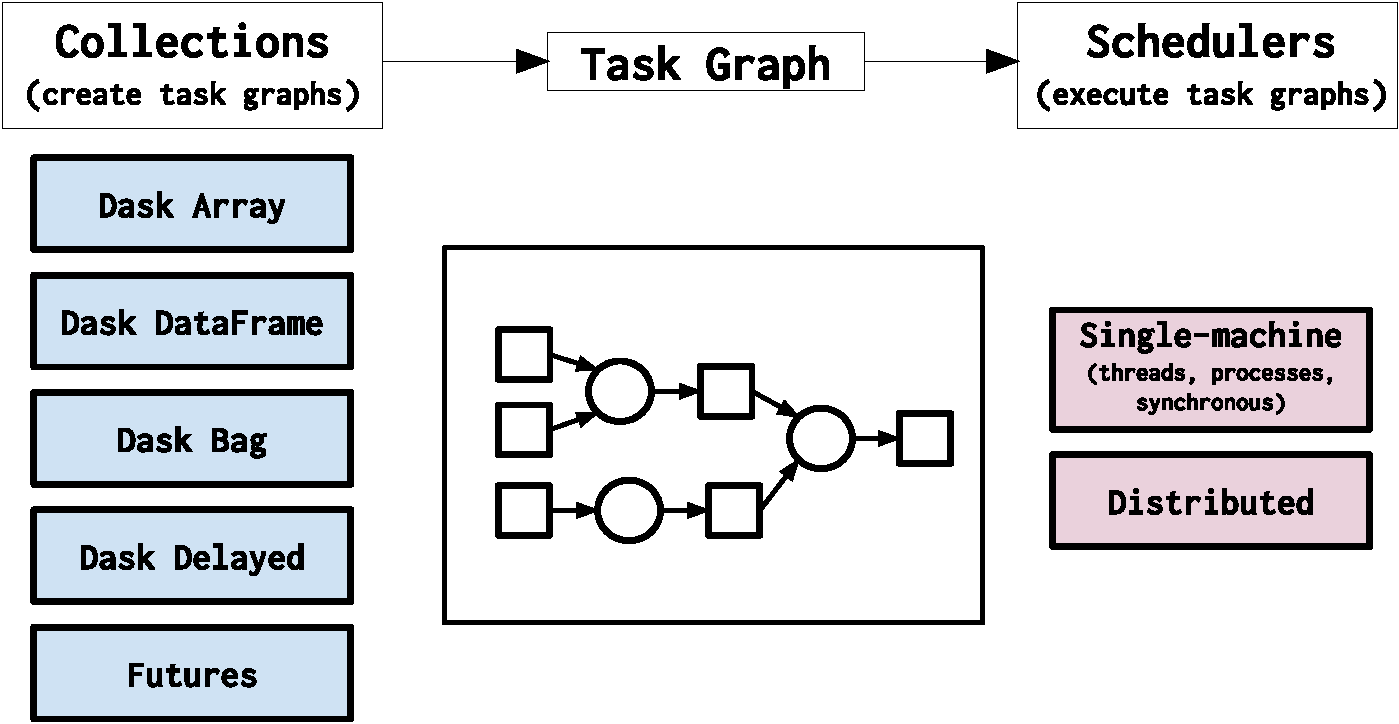
\includegraphics[width=.75\textwidth]{pic/dask-overview}
    \caption{Dask functionality \cite{daskhomepage2020}}
    \label{fig:dask-overview}
\end{figure}



Dask \cite{daskhomepage2020} is a flexible library for parallel computing in Python.
It is composed of these parts:
\begin{enumerate}
\item Scheduler: Dynamic task scheduling optimized for computation. This is similar to Airflow, Luigi, Celery, or Make, but optimized for interactive computational workloads.
\item Graphs: Dask represents parallel computations with task graphs.  Working directly with dask graphs is rare, unless you intend to develop new modules with Dask. Dask graphs are created internally and most users don't ever see a graph. See Section~\ref{sec:DaskComputeGraphs} for an example of a Dask graph.
\item Collections: ``Big Data'' collections like parallel arrays, dataframes, and lists that extend common interfaces like NumPy, Pandas, or Python iterators to larger-than-memory or distributed environments. These parallel collections run on top of dynamic task schedulers.
\end{enumerate}

The graph and collections functionalities are very powerful but not used in the \libraddask{} module. These topics are not further considered here.

Dask installs  conveniently  on a laptop, a desktop or a cluster computer. Dask can scale to a cluster of 100s of machines. This ease of transition between single-machine to moderate cluster enables users to both start simple and grow when necessary.  The \libraddask{} module uses the Dask scheduler to run \libradtran{} on a Linux computer, serving locally or to remote computers.

\section{Dask as Server}

The client Client-Server design pattern is generally used in the context where any number of clients, running on many different (weaker) computers can access the centralised server that is highly optimised to perform a specific set of functions very efficiently.  A common instance of this pattern is in enterprise database systems such as SAP or PeopleSoft. The clients have a small footprint (called 'thin', perhaps even just a browser), with most of the functionality in the main server (often with big databases and high processing capability).

A cloud service is any service made available to users on demand via the Internet from a cloud computing provider's servers as opposed to being provided from a company's own on-premises servers. Cloud services are designed to provide easy, scalable access to applications, resources and services, and are fully managed by a cloud services provider.
In the context of this document, consider the cloud service as a massively parallel computer providing computing and/or storage via the internet.

Dask is neither of the above, it is a technology that enables parallel computation, either on the local computer, on other computers on a private network or even in a cloud service.
Using the Dask distributed module a server-like functionality can be implemented  for doing remote processing in a specialist area --- this is what the current application is doing.

Setting up a distributed computation server with Dask requires that work on the local PC and work on the server be done in Python. Even more strictly, exactly the same versions of Python and all required modules must be installed on all computers.  This requirement stems from Dask's packaging (using pickle or dill) of the code to be executed as well as the data to be used. The combined package of code and data is sent to the remote computer, which returns the resulting data after computation. This model is fundamentally different from conventional servers.

\section{Dask \lstinlineL{Distributed}}



\begin{figure}[htbp]
    \centering
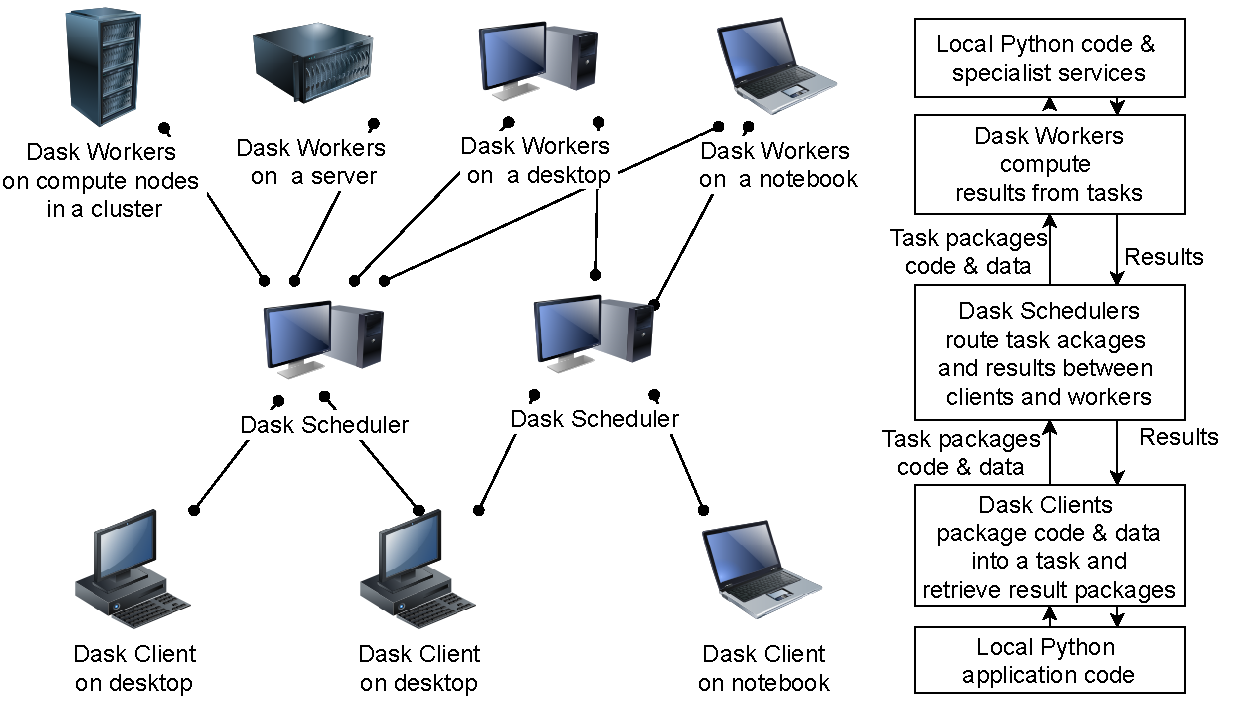
\includegraphics[width=\textwidth]{pic/dask-scheduler}
    \caption{Dask distributed concept}
    \label{fig:dask-scheduler}
\end{figure}

The Dask distributed concept has three major roles:
\begin{enumerate}
    \item Clients: The client resides on a local PC (of any form) which puts together a package of code and data. This package is pickled\footnote{Pickle is a Python way to serialise complex objects into a single package.} and sent to a scheduler.  The client also receives results back from the scheduler. So the client sends task packages and retrieves results.  There can be any number of clients, on any number of computers. One client can communicate with any number of schedulers.

    \item Schedulers: The scheduler listens on a specific port for any client requests. At the same time, the scheduler also polls the workers to keep record of `idle' workers that are available to take on new tasks.  Task packages from clients are routed to available workers for execution. When the worker has completed the task, the scheduler can make it available when the client requests the results. There can be any number of schedulers, on any number of computers. One scheduler can communicate with any number of clients and any number of workers.

    \item Workers: The workers wait for task assignments from the scheduler. When the task package is received it is executed on the worker node CPU. The results are packaged and stored until retrieved by the scheduler.   There can be any number of workers, on any number of computing nodes or computers. One worker can communicate with any number of schedulers.
\end{enumerate}



\begin{figure}[htbp]
    \centering
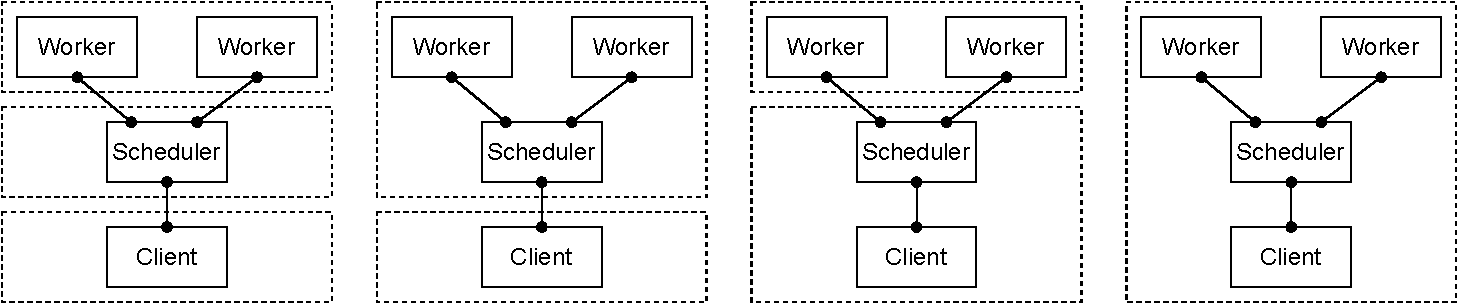
\includegraphics[width=\textwidth]{pic/daskdistriballoc}
    \caption[Dask distributed in different computers configurations]{Dask distributed in different computers configurations. The dotted lines represent different computers}
    \label{fig:daskdistriballoc}
\end{figure}

The Client, the Scheduler and the Worker are all independently running code instances, which could be running on one or more computers. Figure~\ref{fig:daskdistriballoc} shows the options for running the processes. The figure shows the computer hardware boundaries in dashed lines. It is evident that the different processes can run on the same computer, different computers or any mix of computers.  Each computer is identified by an IP address on the network and the network location (IP addresses) of the scheduler and worker computers are specified in the code. Hence, the IP addresses must be known before the code is executed.


\section{Executing User Code}

How does this Dask Distributed fit into the user code?
Imagine the scenario where a Windows user requires a \libradtran{} run, but does not have it compiled for his Windows PC.  Suppose \libradtran{} is available on a Linux computer somewhere on the network. The Linux computer can be single computer in the office next door, or it can be a server on the local network or even in a cloud service.

The user Python application sets up a task package containing some Python code to run \libradtran{} on the remote computer and the input files for the run. The package and execution proceeds from user application code to the Dask client on the local PC, to the scheduler, to the worker (the worker then does some work on the data), the results are then sent back to the scheduler, back to the client, and finally back to the  user code, where the results are processed.  This process can be followed for  a single \libradtran{} run or it can be for thousands of runs, where each run is executed on one of many different workers.  The workers run concurrently on a cluster or on multiple cores in a local CPU.

Once the Dask distributed channel is set up, the user has no further action than to set up the task package.  The distribution and execution is all taken care of by Dask.  The price to be paid for this convenience is setting up the scheduler and worked environments, which is relatively small.  Of course, setting up \libradtran{}  must be done anyway, either on the local or remote computer, so there is no penalty here. In fact, building \libradtran{}  on a Linux PC is relatively simple and quick.

How does the worker know what processing is required?
The package delivered to the worker contains Python code and the input data.
The worker simply executes the Python code in the package, on the data in the package.
The package code can be only Python code, such as a Python machine learning algorithm, but the Python code can also execute other executable codes (such as \libradtran{}) on the worker node. The process to execute other codes will be described later in this report.

\section{Serialisation}

\begin{figure}[htbp]
    \centering
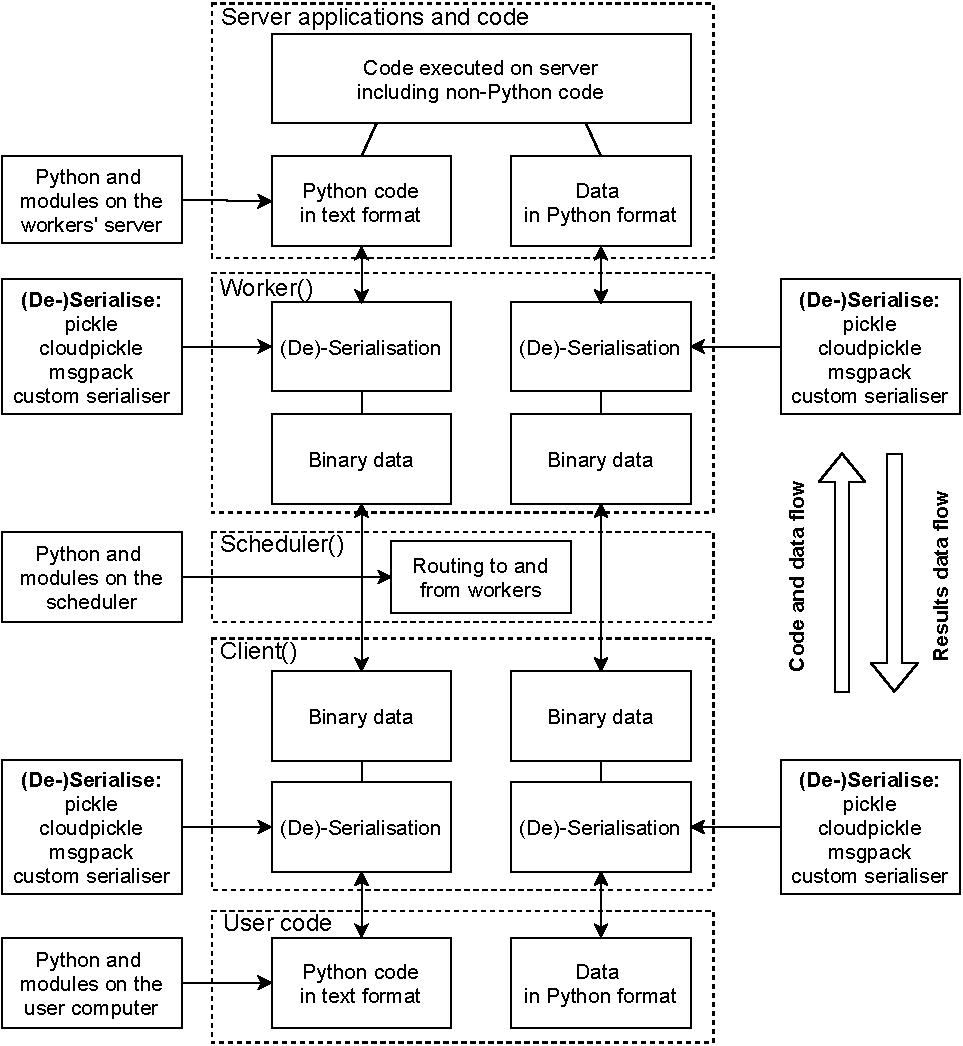
\includegraphics[width=\textwidth]{pic/DaskSerialisation}
    \caption{Dask serialisation}
    \label{fig:DaskSerialisation}
\end{figure}

Passing data between computers requires conversion of the data into a sequence of bytes that can be communicated across the network. The code and data flowing from the user PC to the scheduler and worker must be 'zipped-up'\footnote{The term zip up is used figuratively, it is not implying that the pkzip technology is used.} into a package. This is called serialisation.
Choices made in serialization can affect performance and security.
Dask serialisation is described here: 
\lstinlineN{https://distributed.dask.org/en/latest/serialization.html}.

The standard Python solution to this, Pickle, is often but not always the right solution. Dask uses a number of different serialization schemes in different situations. These are extensible to allow users to control in sensitive situations and also to enable library developers to plug in higher performing serialization solutions. Figure~\ref{fig:DaskSerialisation} shows the serialisation process in Dask.


There are three kinds of messages passed through the Dask network:

\begin{enumerate}
    \item Small administrative messages like ``Worker A has finished task X'' or ``I'm running out of memory''. These are always serialized with \lstinlineN{msgpack}.
    \item  Movement of program data, such as Numpy arrays and Pandas dataframes. This uses a combination of pickle, cloudpickle, msgpack, and custom per-type serialisers that come with Dask.
    \item Computational tasks (Python code) like \lstinlineN{f(x)} that are defined and serialized on client processes and deserialized and run on worker processes. These are serialized using a fixed scheme decided on by those libraries. Today this is a combination of pickle and cloudpickle.

\end{enumerate}
You can choose which families you want to use to serialize data and to deserialize data when you create a client.

The various serialisation modules implement compact binary protocols for serializing and de-serializing a Python object structure. These protocols are unique and version specific, which may lead to incompatibilities between the serialised data and the module versions used to deserialise the data. Most of these serialisation module formats are not transportable between versions.

For more information on the pickle module see \\
\lstinlineN{https://docs.python.org/3/library/pickle.html}, and \\
\lstinlineN{https://docs.python.org/2/library/pickle.html}.


\section{Versions}

Careful review of Figure~\ref{fig:DaskSerialisation} indicates that there are potentially three different Python instances: one each in the user computer, the scheduler computer and one in the worker computer\footnote{If all three instances are on the same computer then the same Python is used.}.  The way Dask works is to pass the Python code for execution to the other computer. If these versions differ, there could be complications.  The idea is that the code should execute exactly the same irrespective of which computer it is executed on. Hence the software versions of Python and all the modules used, must be exactly the same on all computers --- even to the bug fix version (the last number in the three-number version number).

Dask should check the versions as default action when the packages are sent around. If the versions are different the user is warned and the processes is stopped. 
If the versions do not match an error report similar to the following may be displayed. 
The Dask software is continuously updated so the format may differ from as it is shown here.

\begin{lstlisting}
distributed.worker - WARNING - Mismatched versions found

distributed
+---------------------------+---------------------------+
|                           | version                   |
+---------------------------+---------------------------+
| This Worker               | 2.11.0+21.g05ca3fb1.dirty |
| scheduler                 | 2.12.0                    |
| tcp://192.168.0.102:64357 | 2.11.0+21.g05ca3fb1.dirty |
+---------------------------+---------------------------+

msgpack
+---------------------------+---------+
|                           | version |
+---------------------------+---------+
| This Worker               | 0.6.1   |
| scheduler                 | 1.0.0   |
| tcp://192.168.0.102:64357 | 0.6.1   |
+---------------------------+---------+
\end{lstlisting}

or 

\begin{lstlisting}
ValueError: Mismatched versions found

cloudpickle
+------------------------+---------+
|                        | version |
+------------------------+---------+
| client                 | 0.5.3   |
| scheduler              | 0.5.2   |
| tcp://100.96.1.5:36964 | 0.5.2   |
| tcp://100.96.1.6:38415 | 0.5.2   |
| tcp://100.96.2.6:44389 | 0.5.2   |
| tcp://100.96.2.7:39214 | 0.5.2   |
| tcp://100.96.2.8:40317 | 0.5.2   |
+------------------------+---------+

dask
+------------------------+---------+
|                        | version |
+------------------------+---------+
| client                 | 0.18.2  |
| scheduler              | 0.17.4  |
| tcp://100.96.1.5:36964 | 0.17.4  |
| tcp://100.96.1.6:38415 | 0.17.4  |
| tcp://100.96.2.6:44389 | 0.17.4  |
| tcp://100.96.2.7:39214 | 0.17.4  |
| tcp://100.96.2.8:40317 | 0.17.4  |
+------------------------+---------+
\end{lstlisting}

If the process does not work correctly, check for the versions by using \\
\lstinlineN{client.get_versions(check=True)},\\
 that returns the current versions in a json file.

\begin{lstlisting}
{'scheduler': {'host': (('python', '3.7.6.final.0'),
   ('python-bits', 64),
   ('OS', 'Windows'),
   ('OS-release', '7'),
   ('machine', 'AMD64'),
   ('processor', 'Intel64 Family 6 Model 94 Stepping 3, GenuineIntel'),
   ('byteorder', 'little'),
   ('LC_ALL', 'None'),
   ('LANG', 'None')),
  'packages': {'dask': '2.12.0',
   'distributed': '2.12.0',
   'msgpack': '0.6.1',
   'cloudpickle': '1.3.0',
   'tornado': '6.0.4',
   'toolz': '0.10.0',
   'numpy': '1.18.1',
   'lz4': None,
   'blosc': None}},
 'workers': {'tcp://127.0.0.1:63694': {'host': (('python', '3.7.6.final.0'),
    ('python-bits', 64),
    ('OS', 'Windows'),
    ('OS-release', '7'),
    ('machine', 'AMD64'),
    ('processor', 'Intel64 Family 6 Model 94 Stepping 3, GenuineIntel'),
    ('byteorder', 'little'),
    ('LC_ALL', 'None'),
    ('LANG', 'None')),
   'packages': {'dask': '2.12.0',
    'distributed': '2.12.0',
    'msgpack': '0.6.1',
    'cloudpickle': '1.3.0',
    'tornado': '6.0.4',
    'toolz': '0.10.0',
    'numpy': '1.18.1',
    'lz4': None,
    'blosc': None}}},
 'client': {'host': [('python', '3.7.6.final.0'),
   ('python-bits', 64),
   ('OS', 'Windows'),
   ('OS-release', '7'),
   ('machine', 'AMD64'),
   ('processor', 'Intel64 Family 6 Model 94 Stepping 3, GenuineIntel'),
   ('byteorder', 'little'),
   ('LC_ALL', 'None'),
   ('LANG', 'None')],
  'packages': {'dask': '2.12.0',
   'distributed': '2.12.0',
   'msgpack': '0.6.1',
   'cloudpickle': '1.3.0',
   'tornado': '6.0.4',
   'toolz': '0.10.0',
   'numpy': '1.18.1',
   'lz4': None,
   'blosc': None}}}
\end{lstlisting}

The solution to this problem is to ensure that the same versions are present on all computers.
See Section~\ref{sec:Additionalpackages} on installing specific package versions.




\section{Dask Experiments}
\label{sec:DaskExperiments}

The rest of this chapter is an extract from this notebook:\\
\lstinline{https://github.com/NelisW/miscellania/blob/master/dask/Dask-Experiments.ipynb}


\subsection{Setting Up}
\label{sec:SettingUp}

The following page explain in more detail how to set up Dask on a variety of local and distributed hardware.
\lstinline{https://docs.dask.org/en/latest/setup.html}


There are two ways to set up Dask on a local computer. Both of these ways are explored in the notebook.
Setting up on a local computer is important to grasp the concepts even if the end objective is to use a multi PC configuration.


There are several multi-computer set up techniques. This document explores two techniques: manual set up and SSH set up.



\begin{lstlisting}[style=incellstyle]
from dask.distributed import Client, LocalCluster

\end{lstlisting}


\subsection{Single Machine (local PC)}
\label{sec:SingleMachinelocalPC}

The \verb+dask.distributed+ scheduler works well on a single machine. It is sometimes preferred over the default scheduler. 
You can create a \verb+dask.distributed+ scheduler by importing and creating a Client with no arguments. This overrides whatever default was previously set.  In the context of this section, the word distributed is understood to be distributed programmatically on the local physical computer (not distributed in the physical sense).


The \verb+Client()+ call used here  is shorthand for creating a \verb+LocalCluster+ and then passing that to your client.
You may want to look at the wider range  keyword arguments available on \verb+LocalCluster+ to understand the options available to you on handling the mixture of threads and processes, like specifying explicit ports, and so on. For example, if you use the \verb+localCluster+ approach you can set the number of workers.


Note that \verb+Client()+ and \verb+LocalCluster()+ take many optional arguments, to configure the server.


You can navigate to \verb+http://localhost:8787/status+ to see the diagnostic dashboard if you have Bokeh installed.


Once the local client is started it will start a local cluster, but all working on the local computer.


The \verb+client.scheduler\_info()+ command provides information about the client, server and worker setup.


The \verb+client.shutdown()+ command can be used to shut down the client on the server


\lstinline{https://docs.dask.org/en/latest/setup/single-distributed.html }


\lstinline{https://distributed.dask.org/en/latest/api.html#distributed.Client}


Dask is not the only means to do parallel processing.  See also this tutorial on multiprocessing.


\lstinline{https://sebastianraschka.com/Articles/2014\_multiprocessing.html}



\begin{lstlisting}[style=incellstyle]
# to use use local host
useSimpleClient = True

if useSimpleClient:
    # simplified setup, less control
    client = Client() 
else:
    # Setup a local cluster, more control
    # By default this sets up 1 worker per core    
    cluster = LocalCluster(n_workers=1)
    client = Client(cluster)

client.get_versions(check=True)

client
\end{lstlisting}

\begin{center}

\begin{normalsize}

\begin{tabular}{|c|c|}
\hline
Client

  Scheduler: tcp://127.0.0.1:64865
  Dashboard: http://127.0.0.1:8787/status&Cluster

  Workers: 4
  Cores: 8
  Memory: 34.00 GB\\\hline

\end{tabular}
\end{normalsize}
\end{center}


\begin{lstlisting}[style=incellstyle]
client.scheduler_info()
\end{lstlisting}


\begin{lstlisting}[style=outcellstyle]
{'type': 'Scheduler',
 'id': 'Scheduler-e40d7349-ee4d-481f-b416-bc9b75b87b92',
 'address': 'tcp://127.0.0.1:64865',
 'services': {'dashboard': 8787},
 'workers': {'tcp://127.0.0.1:64887': {'type': 'Worker',
   'id': 3,
   'host': '127.0.0.1',
   'resources': {},
   'local_directory': 'V:\\work\\WorkN\\miscellania\\dask\\dask-worker-space\\worker-sz1aoteq',
   'name': 3,
   'nthreads': 2,
   'memory_limit': 8500740096,
   'last_seen': 1586869485.3058014,
   'services': {},
   'metrics': {'cpu': 0.0,
    'memory': 52654080,
    'time': 1586869485.2592325,
    'read_bytes': 0.0,
    'write_bytes': 0.0,
    'executing': 0,
    'in_memory': 0,
    'ready': 0,
    'in_flight': 0,
    'bandwidth': {'total': 100000000, 'workers': {}, 'types': {}}},
   'nanny': 'tcp://127.0.0.1:64868'},
  'tcp://127.0.0.1:64889': {'type': 'Worker',
   'id': 2,
   'host': '127.0.0.1',
   'resources': {},
   'local_directory': 'V:\\work\\WorkN\\miscellania\\dask\\dask-worker-space\\worker-a3868zvm',
   'name': 2,
   'nthreads': 2,
   'memory_limit': 8500740096,
   'last_seen': 1586869485.3589983,
   'services': {},
   'metrics': {'cpu': 0.0,
    'memory': 52600832,
    'time': 1586869485.3125384,
    'read_bytes': 0.0,
    'write_bytes': 0.0,
    'executing': 0,
    'in_memory': 0,
    'ready': 0,
    'in_flight': 0,
    'bandwidth': {'total': 100000000, 'workers': {}, 'types': {}}},
   'nanny': 'tcp://127.0.0.1:64870'},
  'tcp://127.0.0.1:64890': {'type': 'Worker',
   'id': 1,
   'host': '127.0.0.1',
   'resources': {},
   'local_directory': 'V:\\work\\WorkN\\miscellania\\dask\\dask-worker-space\\worker-jou7s9bk',
   'name': 1,
   'nthreads': 2,
   'memory_limit': 8500740096,
   'last_seen': 1586869485.3625963,
   'services': {},
   'metrics': {'cpu': 0.0,
    'memory': 52740096,
    'time': 1586869485.3174865,
    'read_bytes': 0.0,
    'write_bytes': 0.0,
    'executing': 0,
    'in_memory': 0,
    'ready': 0,
    'in_flight': 0,
    'bandwidth': {'total': 100000000, 'workers': {}, 'types': {}}},
   'nanny': 'tcp://127.0.0.1:64869'},
  'tcp://127.0.0.1:64893': {'type': 'Worker',
   'id': 0,
   'host': '127.0.0.1',
   'resources': {},
   'local_directory': 'V:\\work\\WorkN\\miscellania\\dask\\dask-worker-space\\worker-djqrx1np',
   'name': 0,
   'nthreads': 2,
   'memory_limit': 8500740096,
   'last_seen': 1586869485.4007897,
   'services': {},
   'metrics': {'cpu': 0.0,
    'memory': 52621312,
    'time': 1586869485.3620787,
    'read_bytes': 0.0,
    'write_bytes': 0.0,
    'executing': 0,
    'in_memory': 0,
    'ready': 0,
    'in_flight': 0,
    'bandwidth': {'total': 100000000, 'workers': {}, 'types': {}}},
   'nanny': 'tcp://127.0.0.1:64867'}}}
\end{lstlisting}


\begin{lstlisting}[style=incellstyle]
# client.shutdown()
\end{lstlisting}


\begin{lstlisting}[style=incellstyle]
#client.get_versions(check=True)
\end{lstlisting}

There are a few different ways to interact with the cluster through the client:


\begin{enumerate}
\item The Client satisfies most of the standard concurrent.futures - PEP-3148 interface with \verb+.submit+, \verb+.map+ functions and \verb+Future+ objects, allowing the immediate and direct submission of tasks \lstinline{https://docs.python.org/3/library/concurrent.futures.html}.
\item The Client registers itself as the default Dask scheduler, and so runs all dask collections like \verb+dask.array+, \verb+dask.bag+, \verb+dask.dataframe+ and \verb+dask.delayed+
\item The Client has additional methods for manipulating data remotely. See the full API for a thorough list \lstinline{https://distributed.dask.org/en/latest/api.html}.
\end{enumerate}


\subsubsection{Dask Dashboard}
\label{sec:DaskDashboard}

The Dask dashboard is a bokeh-based display of what is taking place in the server and its workers. For this to work the Python bokeh package must be installed.


Workers capture durations associated to tasks. For each task that passes through a worker we record start and stop times for each of the following:


\begin{itemize}
\item Serialization (gray)
\item Dependency gathering from peers (red)
\item Disk I/O to collect local data (orange)
\item Execution times (colored by task)
\end{itemize}

The main way to observe these times is with the task stream plot on the scheduler's /status page where the colors of the bars correspond to the colors listed above.


\lstinline{https://docs.dask.org/en/latest/diagnostics-distributed.html}


\lstinline{https://distributed.dask.org/en/latest/diagnosing-performance.html}


\lstinline{https://medium.com/@kartikbhanot/dask-scheduler-dashboard-understanding-resource-and-task-allocation-in-local-machines-bc5aa60eca6e}


\lstinline{https://www.youtube.com/watch?v=N\_GqzcuGLCY}


There is also a Dask extension for Jupyter notebooks \verb+dask-labextension+.


\lstinline{https://github.com/dask/dask-labextension}



\begin{lstlisting}[style=incellstyle]
# to obtain the dashboard for the client
def clientDashboardURI(client):
    """Extract the bokeh dashboard URI from the client's scheduler info
    """
    
    dashboardURI = client.scheduler_info()['address'].rsplit(':',1)[0]+':'
    dashboardURI += str(client.scheduler_info()['services']['dashboard'])
    
    return dashboardURI.replace('tcp:','http:')

print(clientDashboardURI(client))
\end{lstlisting}


\begin{lstlisting}[style=outcellstyle]
http://127.0.0.1:8787

\end{lstlisting}

Open a browser window with the above URI (for the currently running client). Set the \verb+if+ condition to \verb+True+ and execute the code below to observe the dashboard in action.
The code below is not meaningful it is just meant to keep Dask busy for a while.


While the code is executing, click on the different tabs in the dashboard to learn about the different displays.



\begin{lstlisting}[style=incellstyle]
if False:
    import dask.array as da
    x = da.random.random((10000, 10000,10), chunks=(1000,1000,5))
    y = da.random.random((10000, 10000,10), chunks=(1000,1000,5))
    z = (da.arcsin(x)+da.arccos(y)).sum(axis=(1,2))
    z.compute()
\end{lstlisting}


\subsubsection{Preparing functions}
\label{sec:Preparingfunctions}

Create a few functions that will be used in the examples.



\begin{lstlisting}[style=incellstyle]
# to create simple task to experiment with
def inc(x):
    return x + 1

def add(x, y):
    return x + y

\end{lstlisting}


\subsubsection{Single function calls}
\label{sec:Singlefunctioncalls}

Using the client created above, a single function and a single data (datum?) item will be dispatched to the scheduler and worker. All of the scheduling work is transparent.


We can submit individual function calls with the \verb+client.submit+ method.


The simple example here will execute much faster in normal in-line Python code, the idea here is to show the Dask method.


The \verb+submit+ function returns a \verb+Future+, which refers to a (future) remote result. This result may not yet be completed. Eventually it will complete. The result stays in the remote thread/process/worker until you ask for it back explicitly by calling the \verb+result+ method on the future itself (not a client method as for the map case below).


\lstinline{https://distributed.dask.org/en/latest/client.html}



\begin{lstlisting}[style=incellstyle]
# to create a single future
x1 = client.submit(inc, 10)
print(x1)
\end{lstlisting}


\begin{lstlisting}[style=outcellstyle]
<Future: pending, key: inc-083b5e2ba45c380966bcb963d4544e5e>

\end{lstlisting}


\begin{lstlisting}[style=incellstyle]
# to see what a future looks like
print(x1)
\end{lstlisting}


\begin{lstlisting}[style=outcellstyle]
<Future: finished, type: builtins.int, key: inc-083b5e2ba45c380966bcb963d4544e5e>

\end{lstlisting}


\begin{lstlisting}[style=incellstyle]
# to retrieve a result from a future
x1r = x1.result()
print(x1r)
\end{lstlisting}


\begin{lstlisting}[style=outcellstyle]
11

\end{lstlisting}


\begin{lstlisting}[style=incellstyle]
# to check if a future resets or disappears after its initial retrieval
print(x1)
x1r = x1.result()
print(x1r)
\end{lstlisting}


\begin{lstlisting}[style=outcellstyle]
<Future: finished, type: builtins.int, key: inc-083b5e2ba45c380966bcb963d4544e5e>
11

\end{lstlisting}

You can pass futures as inputs to submit. Dask automatically handles dependency tracking; once all input futures have completed, they will be moved onto a single worker (if necessary), and then the computation that depends on them will be started. You do not need to wait for inputs to finish before submitting a new task; Dask will handle this automatically:



\begin{lstlisting}[style=incellstyle]
# to create a graph of futures
x1 = client.submit(inc, 10)
x2 = client.submit(inc, 10)
print(x1)
print(x2)
xs = client.submit(add,x1,x2)
print(xs)
\end{lstlisting}


\begin{lstlisting}[style=outcellstyle]
<Future: finished, type: builtins.int, key: inc-083b5e2ba45c380966bcb963d4544e5e>
<Future: finished, type: builtins.int, key: inc-083b5e2ba45c380966bcb963d4544e5e>
<Future: pending, key: add-6e6cf98db4b0523bbdc831467bd5720b>

\end{lstlisting}


\begin{lstlisting}[style=incellstyle]
# to print the result of the graph final output
xsr = xs.result()
print(xsr)
\end{lstlisting}


\begin{lstlisting}[style=outcellstyle]
22

\end{lstlisting}


\subsubsection{Multiple function calls}
\label{sec:Multiplefunctioncalls}

Using the client created above, a single function and multiple data items will be dispatched to the scheduler and worker. All of the scheduling work is transparent.


Similar to Python's \verb+map+, you can use \verb+Client.map+ to call the same function and many inputs.


The returns a list of futures.
These results live on the distributed workers.


We can submit tasks on futures. The function will go to the machine where the futures are stored and run on the result once it has completed.In the example below the list of futures is sent to the built-in Python \verb+sum()+ function, which adds the elements of an iterable and returns the sum.



\begin{lstlisting}[style=incellstyle]
# to create a map of input values for a function
futures  = client.map(inc, [2, 4, 6])
for future in futures:
    print(future)
\end{lstlisting}


\begin{lstlisting}[style=outcellstyle]
<Future: pending, key: inc-423e89f2660795305fd6c03c55d1de5d>
<Future: pending, key: inc-98feef5b8b4598158d0e47a6d4acde9d>
<Future: pending, key: inc-d016ddc28876119154a07cfbe98a9ed7>

\end{lstlisting}

The results stay in the remote thread/process/worker until you ask for it back explicitly by calling the client \verb+gather+ method (not the future's result method) because here a list must be processed.



\begin{lstlisting}[style=incellstyle]
# to gather the list of results
futuresr = client.gather(futures)
print(futuresr)
\end{lstlisting}


\begin{lstlisting}[style=outcellstyle]
[3, 5, 7]

\end{lstlisting}


\begin{lstlisting}[style=incellstyle]
# to graph a list of futures into another submit
total = client.submit(sum, futures)
print(total)
 
totalr = total.result()
print(totalr)
\end{lstlisting}


\begin{lstlisting}[style=outcellstyle]
<Future: pending, key: sum-c34d59da0efacac3f60627d03084e274>
15

\end{lstlisting}

\subsubsection{Serialising Code and Data}
\label{sec:SerialisingCodeandData}

In the examples shown above the code and data are serialised in the client before passing on to the scheduler. This can be visualised as shown in Figure~\ref{fig:DaskSerialisation02}.


\begin{figure}[htbp]
    \centering
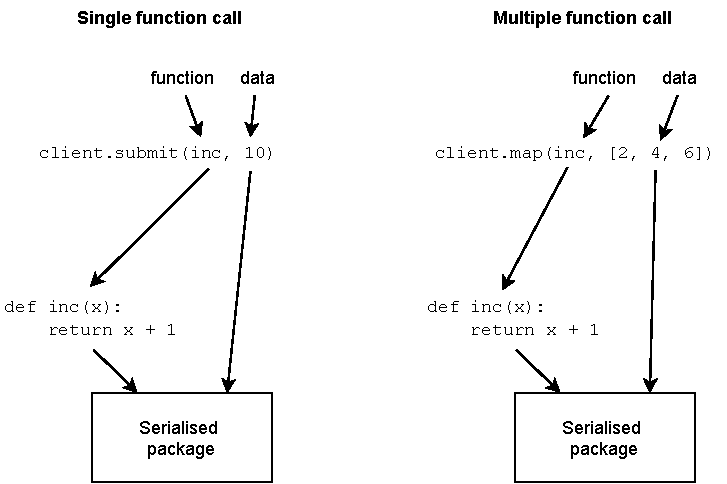
\includegraphics[width=.8\textwidth]{pic/DaskSerialisation02}
    \caption{Dask serialisation and worker execution visualised}
    \label{fig:DaskSerialisation02}
\end{figure}


\subsection{Multiple Machines (local PC and Remote Server(s))}
\label{sec:MultipleMachineslocalPCandRemoteServers}


\subsubsection{Setting up}
\label{sec:Settingup}

For the sake of these discussions suppose the computers have the following  IP addresses (replace with the IP addresses on your system):
\begin{enumerate}
\item Local computer running the \verb+dask.distributed.Client+:  \verb+146.64.202.163+
\item Computer running the scheduler: \verb+146.64.246.94+
\item Computer running the workers: \verb+146.64.246.94+
\end{enumerate}



In this case the scheduler and worker are run on the same server, but could be ran on different computers.


All three computers must have exactly the same versions of Python, dask, pickle, etc., otherwise the following will not work. If required versions are available in a Python environment, the environment must be activated.


The client, scheduler and workers must be able to communicate with each other. This is achieved by using selected ports and IP addresses. The main IP address of interest here is the scheduler IP address which must be made known to the client and the workers, see the example below.

\begin{figure}[htbp]
    \centering
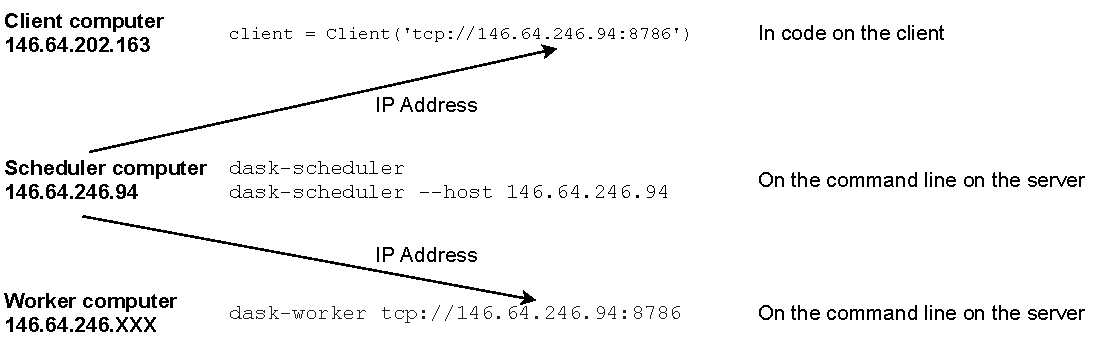
\includegraphics[width=\textwidth]{pic/serverIP}
    \caption{IP port notification in Dask}
    \label{fig:serverIP}
\end{figure}


Start the scheduler and workers:


\begin{enumerate}
\item \textbf{Start the scheduler on the server}. Log in to the server (\lstinline{146.64.246.94}), then activate the Python environment and start the scheduler:

\begin{lstlisting}
conda activate devpy37
dask-scheduler
\end{lstlisting}

If the server already has the necessary Python, dask and pickle versions in the root Python environment there is no need to first activate the Python environment.  In this case the scheduler can be started from any computer by specifying the hostname. So on the local computer the following command will start the scheduler (if versions are correct in the root Python):

\begin{lstlisting}
dask-scheduler --host 146.64.246.94
\end{lstlisting}

Either of the above should start the scheduler:
\begin{lstlisting}[style=tinysize]
(devpy37) username@servername:~$ dask-scheduler
 distributed.scheduler - INFO - -----------------------------------------------
 distributed.scheduler - INFO - Local Directory:    /tmp/scheduler-mxiy5sli
 distributed.scheduler - INFO - -----------------------------------------------
 distributed.scheduler - INFO - Clear task state
 distributed.scheduler - INFO -   Scheduler at:  tcp://146.64.246.94:8786
 distributed.scheduler - INFO -   dashboard at:                     :8787
 distributed.scheduler - INFO - Register worker <Worker 'tcp://146.64.246.94:45347', name: tcp://146.64.246.94:45347, memory: 0, processing: 0>
 distributed.scheduler - INFO - Starting worker compute stream, tcp://146.64.246.94:45347
 distributed.core - INFO - Starting established connection
\end{lstlisting}

\item \textbf{Start the worker on the server}  Log in to the server (\lstinline{146.64.246.94}), then activate the Python environment and start the worker:        

\begin{lstlisting}
dask-worker tcp://146.64.246.94:8786
\end{lstlisting}

where the IP address and port number must correspond to the scheduler IP and port address. This should start the worker task. Note that the dashboard IP address is also given when the workers start. Without explicitly defining the number of processors, this server has 32 cores and 32 GB memory.    

\begin{lstlisting}[style=tinysize]
(devpy37) username@servername:~$ dask-worker tcp://146.64.246.94:8786
distributed.nanny - INFO -         Start Nanny at: 'tcp://146.64.246.94:35459'
distributed.worker - INFO -       Start worker at:  tcp://146.64.246.94:45347
distributed.worker - INFO -          Listening to:  tcp://146.64.246.94:45347
distributed.worker - INFO -          dashboard at:        146.64.246.94:42791
distributed.worker - INFO - Waiting to connect to:   tcp://146.64.246.94:8786
distributed.worker - INFO - -------------------------------------------------
distributed.worker - INFO -               Threads:                         32
distributed.worker - INFO -                Memory:                   33.71 GB
distributed.worker - INFO -       Local Directory: /home/username/dask-worker-space/worker-lz08iq0s
distributed.worker - INFO - -------------------------------------------------
distributed.worker - INFO -         Registered to:   tcp://146.64.246.94:8786
distributed.worker - INFO - -------------------------------------------------
distributed.core - INFO - Starting established connection
\end{lstlisting}

You can also define the number of processors to be used and the threads per processor, see \\ https://stackoverflow.com/questions/49406987/how-do-we-choose-nthreads-and-nprocs-per-worker-in-dask-distributed\\

By default Dask creates a single process with as many threads as you have logical cores on your machine (as determined by \lstinline{multiprocessing.cpu_count()}).
\begin{lstlisting}
dask-worker ... --nprocs 1 --nthreads 8  # assuming you have eight cores
dask-worker ...                          # this is actually the default setting
\end{lstlisting}
Using few processes and many threads per process is good if you are doing mostly numeric workloads, such as are common in Numpy, Pandas, and Scikit-Learn code, which is not affected by Python's Global Interpreter Lock (GIL).
However, if you are spending most of your compute time manipulating Pure Python objects like strings or dictionaries then you may want to avoid GIL issues by having more processes with fewer threads each
\begin{lstlisting}
dask-worker ... --nprocs 8 --nthreads 1
\end{lstlisting}
Based on benchmarking you may find that a more balanced split is better
\begin{lstlisting}
dask-worker ... --nprocs 4 --nthreads 2
\end{lstlisting}
Using more processes avoids GIL issues, but adds costs due to inter-process communication. You would want to avoid many processes if your computations require a lot of inter-worker communication..

So specifying eight processors:
\begin{lstlisting}
dask-worker tcp://146.64.246.94:8786 --nprocs 8
\end{lstlisting}
Starts the workers as follows, each with a different port number (not all the detail shown here):

\begin{lstlisting}
(mordevpy37) dgriffith@nimbus:~/libRadtran/libRadtran-2.0.3/bin$ dask-worker tcp://146.64.246.94:8786 --nprocs 8
distributed.nanny - INFO -         Start Nanny at: 'tcp://146.64.246.94:33671'
distributed.nanny - INFO -         Start Nanny at: 'tcp://146.64.246.94:46725'
distributed.nanny - INFO -         Start Nanny at: 'tcp://146.64.246.94:42509'
distributed.nanny - INFO -         Start Nanny at: 'tcp://146.64.246.94:42983'
distributed.nanny - INFO -         Start Nanny at: 'tcp://146.64.246.94:43735'
distributed.nanny - INFO -         Start Nanny at: 'tcp://146.64.246.94:36947'
distributed.nanny - INFO -         Start Nanny at: 'tcp://146.64.246.94:40075'
distributed.nanny - INFO -         Start Nanny at: 'tcp://146.64.246.94:40495'
...
distributed.worker - INFO -       Start worker at:  tcp://146.64.246.94:36533
distributed.worker - INFO -          Listening to:  tcp://146.64.246.94:36533
distributed.worker - INFO -          dashboard at:        146.64.246.94:43069
distributed.worker - INFO - Waiting to connect to:   tcp://146.64.246.94:8786
distributed.worker - INFO - -------------------------------------------------
distributed.worker - INFO -               Threads:                          4
distributed.worker - INFO -                Memory:                    4.21 GB
distributed.worker - INFO -       Local Directory: /home/dgriffith/libRadtran/libRadtran-2.0.3/bin/dask-worker-space/worker-_0o0qta1
distributed.worker - INFO - -------------------------------------------------
distributed.worker - INFO -         Registered to:   tcp://146.64.246.94:8786
distributed.worker - INFO - -------------------------------------------------
distributed.core - INFO - Starting established connection
...
distributed.worker - INFO -       Start worker at:  tcp://146.64.246.94:46597
distributed.worker - INFO -          Listening to:  tcp://146.64.246.94:46597
distributed.worker - INFO -          dashboard at:        146.64.246.94:33737
distributed.worker - INFO - Waiting to connect to:   tcp://146.64.246.94:8786
distributed.worker - INFO - -------------------------------------------------
distributed.worker - INFO -               Threads:                          4
distributed.worker - INFO -                Memory:                    4.21 GB
distributed.worker - INFO -       Local Directory: /home/dgriffith/libRadtran/libRadtran-2.0.3/bin/dask-worker-space/worker-n0anjq00
distributed.worker - INFO - -------------------------------------------------
distributed.core - INFO - Starting established connection
distributed.worker - INFO -         Registered to:   tcp://146.64.246.94:8786
distributed.worker - INFO - -------------------------------------------------
distributed.core - INFO - Starting established connection
\end{lstlisting}


\item \textbf{Start the client}  When the client is initiated, pass the scheduler IP:port address:

\begin{lstlisting}[style=tinysize]
# to start a local client with a remote scheduler
client = Client('146.64.246.94:8786') 
\end{lstlisting}

To see the Python module versions:
\begin{lstlisting}[style=tinysize]
client.get_versions(check=True)
\end{lstlisting}

\begin{lstlisting}[style=outcellstyle]
{'scheduler': {'host': (('python', '3.7.6.final.0'),
   ('python-bits', 64),
   ('OS', 'Linux'),
   ('OS-release', '4.9.0-8-amd64'),
   ('machine', 'x86_64'),
   ('processor', ''),
   ('byteorder', 'little'),
   ('LC_ALL', 'None'),
   ('LANG', 'en_ZA.UTF-8')),
  'packages': {'dask': '2.12.0',
   'distributed': '2.12.0',
   'msgpack': '0.6.1',
   'cloudpickle': '1.3.0',
   'tornado': '6.0.4',
   'toolz': '0.10.0',
   'numpy': '1.18.1',
   'lz4': None,
   'blosc': None}},
 'workers': {'tcp://146.64.246.94:45347': {'host': (('python',
     '3.7.6.final.0'),
    ('python-bits', 64),
    ('OS', 'Linux'),
    ('OS-release', '4.9.0-8-amd64'),
    ('machine', 'x86_64'),
    ('processor', ''),
    ('byteorder', 'little'),
    ('LC_ALL', 'None'),
    ('LANG', 'en_ZA.UTF-8')),
   'packages': {'dask': '2.12.0',
    'distributed': '2.12.0',
    'msgpack': '0.6.1',
    'cloudpickle': '1.3.0',
    'tornado': '6.0.4',
    'toolz': '0.10.0',
    'numpy': '1.18.1',
    'lz4': None,
    'blosc': None}}},
 'client': {'host': [('python', '3.7.6.final.0'),
   ('python-bits', 64),
   ('OS', 'Windows'),
   ('OS-release', '7'),
   ('machine', 'AMD64'),
   ('processor', 'Intel64 Family 6 Model 94 Stepping 3, GenuineIntel'),
   ('byteorder', 'little'),
   ('LC_ALL', 'None'),
   ('LANG', 'None')],
  'packages': {'dask': '2.12.0',
   'distributed': '2.12.0',
   'msgpack': '0.6.1',
   'cloudpickle': '1.3.0',
   'tornado': '6.0.4',
   'toolz': '0.10.0',
   'numpy': '1.18.1',
   'lz4': None,
   'blosc': None}}}
\end{lstlisting}



To see the Dask scheduler information:
\begin{lstlisting}[style=tinysize]
client.scheduler_info()
\end{lstlisting}

To determine the number of workers:
\begin{lstlisting}[style=tinysize]
len(client.scheduler_info()['workers'])
\end{lstlisting}

\begin{lstlisting}[style=outcellstyle]
4
\end{lstlisting}


\begin{lstlisting}[style=outcellstyle]
{'type': 'Scheduler',
 'id': 'Scheduler-c18c6181-421b-4826-aea7-b1bba21efeb0',
 'address': 'tcp://146.64.246.94:8786',
 'services': {'dashboard': 8787},
 'workers': {'tcp://146.64.246.94:45347': {'type': 'Worker',
   'id': 'tcp://146.64.246.94:45347',
   'host': '146.64.246.94',
   'resources': {},
   'local_directory': '/home/dgriffith/dask-worker-space/worker-lz08iq0s',
   'name': 'tcp://146.64.246.94:45347',
   'nthreads': 32,
   'memory_limit': 33712070656,
   'last_seen': 1586869487.8488212,
   'services': {'dashboard': 42791},
   'metrics': {'cpu': 2.0,
    'memory': 107896832,
    'time': 1586869487.3504004,
    'read_bytes': 16650.21565100753,
    'write_bytes': 1014.9159528091943,
    'num_fds': 25,
    'executing': 0,
    'in_memory': 0,
    'ready': 0,
    'in_flight': 0,
    'bandwidth': {'total': 100000000, 'workers': {}, 'types': {}}},
   'nanny': 'tcp://146.64.246.94:35459'}}}
\end{lstlisting}

\end{enumerate}



\subsubsection{Running workers remotely}
\label{sec:Runningworkersremotely}

Now execute the same graph as on the single computer before, but now on the remote server.


To see if the server is running, put the \verb+client()+ call in a Python exception.



\begin{lstlisting}[style=incellstyle]
# to run the graph on a remove server

try:
    client = Client('tcp://146.64.246.94:8786', timeout='2s')
    x1 = client.submit(inc, 10)
    x2 = client.submit(inc, 10)
    print(x1)
    print(x2)
    xs = client.submit(add,x1,x2)
    print(xs)
    # to print the result of the graph final output
    xsr = xs.result()
    print(xsr)
except TimeoutError:
    print('dask scheduler server is not responding, probably not running.')

\end{lstlisting}


\begin{lstlisting}[style=outcellstyle]
<Future: pending, key: inc-083b5e2ba45c380966bcb963d4544e5e>
<Future: pending, key: inc-083b5e2ba45c380966bcb963d4544e5e>
<Future: pending, key: add-6e6cf98db4b0523bbdc831467bd5720b>
22

\end{lstlisting}


\subsubsection{Debugging}
\label{sec:Debugging}

If the scheduler fails to start with messages such as shown below, check to see


\begin{enumerate}
\item If starting the scheduler remotely with \verb+dask-scheduler --host 146.64.246.94+: Does the server's root Python have the correct software and versions? If the scheduler is started remotely the server's root Python is used.
\item If the server is started locally on the server with \verb+dask-scheduler+: Does the currently active Python environment (root or other) have the correct software and versions?
\end{enumerate}

\begin{lstlisting}[style=tinysize]
dask-scheduler --host 146.64.202.118
distributed.scheduler - INFO - -----------------------------------------------
distributed.dashboard.proxy - INFO - To route to workers diagnostics web server please install jupyter-server-proxy: python -m pip install jupyter-server-proxy
distributed.scheduler - INFO - Local Directory: C:\Users\NWillers\AppData\Local\Temp\scheduler-b856sir6
distributed.scheduler - INFO - -----------------------------------------------
distributed.scheduler - INFO - Clear task state
Traceback (most recent call last):
  File "C:\ProgramData\Anaconda3\lib\site-packages\distributed\cli\dask\_scheduler.py", line 237, in main
    loop.run\_sync(run)
  File "C:\ProgramData\Anaconda3\lib\site-packages\tornado\ioloop.py", line 532, in run\_sync
    return future\_cell[0].result()
  File "C:\ProgramData\Anaconda3\lib\site-packages\distributed\cli\dask\_scheduler.py", line 233, in run
    await scheduler
  File "C:\ProgramData\Anaconda3\lib\site-packages\distributed\scheduler.py", line 1424, in start
    await self.listen(addr, listen\_args=self.listen\_args)
  File "C:\ProgramData\Anaconda3\lib\site-packages\distributed\core.py", line 319, in listen
    connection\_args=listen\_args,
  File "C:\ProgramData\Anaconda3\lib\site-packages\distributed\comm\core.py", line 170, in \_
    await self.start()
  File "C:\ProgramData\Anaconda3\lib\site-packages\distributed\comm\tcp.py", line 411, in start
    self.port, address=self.ip, backlog=backlog
  File "C:\ProgramData\Anaconda3\lib\site-packages\tornado\netutil.py", line 174, in bind\_sockets
    sock.bind(sockaddr)
OSError: [WinError 10049] The requested address is not valid in its context
\end{lstlisting}





 % Dask
% -*- TeX -*- -*- UK -*- -*- Soft -*-


\chapter{\libradtran{}}
\label{chap:libRadtran}


\section{\libradtran{} Overview}

From \cite{EmdeLibRadtran2016}:
``\libradtran{} is a widely used software package for
radiative transfer calculations. It allows one to compute (polarized) radiances, irradiance, and actinic fluxes in the solar and thermal spectral regions. \libradtran{} has been used
for various applications, including remote sensing of clouds,
aerosols and trace gases in the Earth’s atmosphere, climate
studies, e.g., for the calculation of radiative forcing due to
different atmospheric components, for UV forecasting, the
calculation of photolysis frequencies, and for remote sensing
of other planets in our solar system. The package has been
described in Mayer and Kylling (2005) \cite{libRadtran2005}. Since then several
new features have been included, for example polarization,
Raman scattering, a new molecular gas absorption parameterization, and several new parameterizations of cloud and
aerosol optical properties. Furthermore, a graphical user interface is now available, which greatly simplifies the usage
of the model, especially for new users. This paper gives an
overview of \libradtran{} version 2.0.1 with a focus on new features. Applications including these new features are provided
as examples of use. A complete description of \libradtran{} and
all its input options is given in the user manual included in
the \libradtran{} software package, which is freely available at
\lstinline{http://www.libradtran.org}.''

See also 
\cite{libRadtran2005,libRadTranUserGuide2012,libRadtranDownload2020,libRadtranmuenchen2020}.


\section{Obtaining and Building \libradtran{}}

\subsection{System Reference}
For reference purposes this installation was done on the following Linux system: Debian 4.9.110, running the 4.9.0-8-amd64 Linux kernel.
\begin{lstlisting}[style=tinysize]
(devpy27) dgriffith@servername:~/libRadtran/libRadtran-2.0.3/examples$ uname -a
Linux servername 4.9.0-8-amd64 #1 SMP Debian 4.9.110-3+deb9u6 (2018-10-08) x86_64 GNU/Linux
\end{lstlisting}

\subsection{Downloading  \libradtran{}}

Download \libradtran{} and the optional additional files/modules from\\
\lstinline{http://www.libradtran.org/doku.php?id=download}\\
For our application the REPTRAN absorption parameterization data was required, but it may differ between different sites.


\subsection{Create the server account and software}

\begin{enumerate}
\item Create a user account on the server from which libRadtran is served. This is a standard Linux admin task.  For the present case assume the account name is \lstinline{dgriffith}.

\item Download libRadtran from \lstinline{http://www.libradtran.org/doku.php?id=download} and follow the installation instructions. The instructions are repeated below.      In this case \libradtran{} version 2.0.3 is downloaded and installed.

\item Copy the downloaded file to the folder where it must be installed. Unzipping the compressed tar file with the following command will create a folder \lstinline{libRadtran-2.0.3}

\begin{lstlisting}
    tar -xvf  libradtran-2.0.3.tar.gz
\end{lstlisting}
\item The \libradtran{} installation, building, and testing requires Python 2.7 (installation will fail if Python 3 is used).  If necessary, install Python 2.7 in a conda environment in order to proceed with the \libradtran{} installation.  For the purpose of this discussion we assume that the Python 2.7 environment is named \lstinline{devpy27}.

\begin{lstlisting}
    conda create --name devpy27 python=2.7 anaconda
\end{lstlisting}

\item Compile the distribution by doing the following:

\begin{lstlisting}
    conda activate devpy27
    cd libRadtran-2.0.3
    ./configure
    make
\end{lstlisting}
\item Test the program, (make sure to use GNU make):

\begin{lstlisting}
    conda activate devpy27
    make check 
\end{lstlisting}
 As the test progresses the test results will display in the terminal (the display shown here has been shortened):


\begin{lstlisting}[style=tinysize]
(base) dgriffith@servername:~/libRadtran/libRadtran-2.0.3$ conda activate devpy27
(devpy27) dgriffith@servername:~/libRadtran/libRadtran-2.0.3$ make check
for dir in examples src_py libsrc_c libsrc_f src GUI lib; do make -C $dir all || exit $?; done
make[1]: Entering directory '/home/dgriffith/libRadtran/libRadtran-2.0.3/examples'

...

make[1]: Entering directory '/home/dgriffith/libRadtran/libRadtran-2.0.3/test'
/usr/bin/perl test.pl
Running various libRadtran tests. This may take some time....

The numbers in the parenthesis behind the name of the tests are:
 1st number:  The lower absolute limit of values included in the test.
              Values in the output less than limit are ignored.
 2nd number:  The maximum difference allowed between local test
              results and the standard results (in percentage).

If this is still unclear, check the source in test/test.pl.in.

make_slitfunction test
make_slitfunction (0.00001,   0.1)............................................. ok.
All make_slitfunction tests succeeded.
make_angresfunc test
make_angresfunc (0.00001,   0.1)............................................... ok.
All make_angresfunc tests succeeded.
angres test
angres (0.00001,   0.1)........................................................ ok.
All angres tests succeeded.
Some \lstinline{uvspec} tests
uvspec simple (0.00001,   0.1)................................................. ok.
disort clear sky (0.00001,   0.1).............................................. ok.
disort aerosol (0.00001,   0.1)................................................ ok.
disort aerosol moments (0.00001,   0.1)........................................ ok.
disort aerosol refractive index (0.00001,   0.1)............................... ok.
disort BRDF Ross-Li (0.00050,   0.1)........................................... ok.
disort water cloud (0.00001,   0.1)............................................ ok.
disort SO2 (0.00001,   0.1).................................................... ok.
disort radiances (0.00001,   0.3).............................................. ok.
disort SCIAMACHY HG approximation (0.00001,   0.3)............................. ok.
disort aerosol (0.00001,   0.1)................................................ ok.
disort wc Legendre moments (0.00001,   0.1).................................... ok.
disort water and ice clouds (0.00001,   0.2)................................... ok.
disort cloud overlap random (0.00001,   0.2)................................... ok.
disort cloud overlap maximum-random (0.00001,   0.2)........................... ok.
disort cloud overlap maximum (0.00001,   0.2).................................. ok.
disort, albedo and altitude map (0.00001,   0.7)............................... ok.
disort BRDF (0.00050,   0.1)................................................... ok.
disort BRDF Hapke (0.00050,   0.1)............................................. ok.
disort BRDF AMBRALS (0.00050,   0.1)........................................... ok.
disort BRDF AMBRALS file (0.00050,   0.1)...................................... ok.
twostr aerosol and water cloud (0.00001,   0.1)................................ ok.
twostrpp aerosol and water cloud (0.00001,   0.1).............................. ok.
c_twostr aerosol and water cloud (0.00001,   0.1).............................. ok.
rodents aerosol and water cloud (0.00001,   0.1)............................... ok.
rodents aerosol and water cloud, zout (0.00001,   0.1)......................... ok.
rodents aerosol and water cloud, zout, thermal (0.00001,   0.1)................ ok.
single scattering lidar, water cloud (0.00001,   0.1).......................... ok.
twostrebe aerosol and water cloud (0.00001,   0.1)............................. ok.
twomaxrand water cloud (0.00001,   0.1)........................................ ok.
twomaxrand wc/ic cloud (0.00001,   0.1)........................................ ok.
polradtran (0.00001,   0.1).................................................... ok.
profiles 1 (0.00001,   0.2).................................................... ok.
profiles 2 (0.00001,   0.1).................................................... ok.
profiles 3 (0.00001,   0.1).................................................... ok.
profiles 4 (0.00001,   0.1).................................................... ok.
radiosonde (0.00001,   0.4).................................................... ok.
redistribution (0.00001,   0.1)................................................ ok.
AVHRR [Kratz, 1995], channel 1, solar (0.00001,   0.1)......................... ok.
AVHRR [Kratz, 1995], channel 2, solar (0.00100,   0.1)......................... ok.
AVHRR [Kratz, 1995], channel 3, solar (0.00001,   0.1)......................... ok.
AVHRR [Kratz, 1995], channel 3, thermal (0.00001,   0.1)....................... ok.
AVHRR [Kratz, 1995], channel 4, thermal (0.00001,   0.1)....................... ok.
AVHRR [Kratz, 1995], channel 5, thermal (0.00001,   0.1)....................... ok.
correlated-k [Kato et al., 1999], twostr (0.00100,   0.1)...................... ok.
correlated-k, new Kato tables, twostr (0.00100,   0.1)......................... ok.
correlated-k [Fu and Liou, 1992/93], disort (0.01000,   1.5)................... ok.
correlated-k [Fu and Liou, 1992/93], ice clouds (0.01000,   1.5)............... ok.
Fu and Liou, thermal irradiance, disort (0.00001,   0.9)....................... ok.
LOWTRAN absorption parameterization (0.00001,   2.2)........................... ok.
LOWTRAN absorption parameterization, thermal (0.00001,   1.0).................. ok.
SSRadar Test (0.01000,   0.0).................................................. ok.
atmospheric reflectivity (0.00001,   0.1)...................................... ok.
IPA and correlated_k (0.00100,   0.2).......................................... ok.
cloudcover and correlated_k (0.00100,   1.8)................................... ok.
cloudcover, correlated_k and redistribution (0.00100,   1.8)................... ok.
wc_ipa_files and correlated_k (0.00100,   0.1)................................. ok.
wc_ipa_files, correlated_k and redistribution (0.00100,   0.1)................. ok.
wc_ipa_files, ic_ipa_files and redistribution (0.00001,   0.1)................. ok.
heating rates and wc_ipa_files (0.00100,   0.2)................................ ok.
cooling rates and wc_ipa_files (0.00100,   1.9)................................ ok.
transmittance_wl_file (0.00100,   0.1)......................................... ok.
raman (0.10000,   0.1)......................................................... ok.
fluorescence (0.10000,   0.1).................................................. ok.
reptran_thermal (0.01000,   0.1)............................................... ok.
reptran_solar (0.01000,   0.2)................................................. ok.
tzs (0.01000,   0.1)........................................................... ok.
disort_spherical_albedo (0.01000,   0.1)....................................... ok.
MYSTIC polarisation (0.00001,   3.0)........................................... ok.
MYSTIC polarized surface reflection (BPDF) (0.00001,   1.0)....................    1 serious differences.  Maximum difference:   1.030000%. Absolute values (test,ans): (-7.743240e-03, -7.663602e-03).
MYSTIC backward polarized surface reflection (BPDF) (0.00001,   1.0)........... ok.
MYSTIC spectral importance sampling (REPTRAN) (0.00001,   5.0)................. ok.
MYSTIC boxairmass factor (0.00001,   1.0)...................................... ok.
MYSTIC spherical (0.00001,   2.0).............................................. ok.
NCA 1.0 (0.00001,   0.1)....................................................... ok.
NCA 2.0 cuboid (0.00001,   0.1)................................................ ok.
NCA 2.0 triangle (0.00001,   0.1).............................................. ok.
1 of the \lstinline{uvspec} tests failed.
make[1]: Leaving directory '/home/dgriffith/libRadtran/libRadtran-2.0.3/test'
(devpy27) dgriffith@servername:~/libRadtran/libRadtran-2.0.3$
\end{lstlisting}

From the above test report it is evident that the \lstinline{MYSTIC polarized surface reflection (BPDF)} test had a result error difference of 1.03\%.
All the other tests passed.

\end{enumerate}

\section{Introductory Example Use}

The following is taken (with some adaptation) from \\
\lstinline{http://www.libradtran.org/doku.php?id=basic_usage}

Those users who are not familiar with the predecessor of \libradtran(), \lstinline{uvspec}, please note the following: The central program of the package is an executable called \lstinline{uvspec} which can be found in the bin directory. If you are interested in a user-friendly program for radiative transfer calculations, \lstinline{uvspec} is the software you want to become familiar with. A description of \lstinline{uvspec} is provided in the first part of the manual. Examples of its use, including various input files and corresponding output files for different atmospheric conditions, are provided in the examples directory. For a quick try of \lstinline{uvspec} go to the examples directory and run \lstinline{uvspec}:

\begin{lstlisting}
    cd libRadtran-2.0.3/examples
    ../bin/uvspec < UVSPEC_CLEAR.INP > test.out
\end{lstlisting}



The input file for this example run is given in \lstinline{UVSPEC_CLEAR.INP}

\begin{lstlisting}[style=tinysize]
                         # Location of atmospheric profile file. 
atmosphere_file ../data/atmmod/afglus.dat
                         # Location of the extraterrestrial spectrum
source solar ../data/solar_flux/atlas_plus_modtran
mol_modify O3 300. DU    # Set ozone column
day_of_year 170          # Correct for Earth-Sun distance
albedo 0.2               # Surface albedo
sza 32.0                 # Solar zenith angle
rte_solver disort        # Radiative transfer equation solver
number_of_streams  6     # Number of streams
wavelength 299.0 341.0   # Wavelength range [nm]
slit_function_file ../examples/TRI_SLIT.DAT
                         # Location of slit function
spline 300 340 1         # Interpolate from first to last in step

quiet
\end{lstlisting}

This input file yields the following output file (the details of which you can decipher from the \libradtran{} User Guide \cite{libRadTranUserGuide2019}):

\begin{lstlisting}[style=tinysize]
  300.000  2.763049e+00  3.087059e+00  1.170022e+00  2.592736e-01  4.777781e-01  1.862147e-01 
  301.000  5.223602e+00  5.888303e+00  2.222381e+00  4.901621e-01  9.168083e-01  3.537029e-01 
  302.000  6.212306e+00  7.024819e+00  2.647425e+00  5.829381e-01  1.098937e+00  4.213508e-01 
  303.000  1.499798e+01  1.709326e+01  6.418247e+00  1.407351e+00  2.687637e+00  1.021496e+00 
  304.000  1.731212e+01  1.968946e+01  7.400318e+00  1.624501e+00  3.108258e+00  1.177797e+00 
  305.000  2.666450e+01  3.052658e+01  1.143822e+01  2.502091e+00  4.841135e+00  1.820449e+00 
  306.000  2.714423e+01  3.094949e+01  1.161874e+01  2.547107e+00  4.925832e+00  1.849181e+00 
  307.000  3.892420e+01  4.444759e+01  1.667436e+01  3.652493e+00  7.100925e+00  2.653807e+00 
  308.000  4.928456e+01  5.616349e+01  2.108961e+01  4.624668e+00  9.003217e+00  3.356516e+00 
  309.000  4.968203e+01  5.629452e+01  2.119531e+01  4.661965e+00  9.051084e+00  3.373338e+00 
  310.000  5.282494e+01  5.981413e+01  2.252781e+01  4.956883e+00  9.651869e+00  3.585413e+00 
  311.000  9.116537e+01  1.021252e+02  3.865812e+01  8.554597e+00  1.652179e+01  6.152631e+00 
  312.000  8.539021e+01  9.519187e+01  3.611642e+01  8.012679e+00  1.544426e+01  5.748106e+00 
  313.000  1.008859e+02  1.116138e+02  4.249995e+01  9.466736e+00  1.815837e+01  6.764078e+00 
  314.000  1.140307e+02  1.247804e+02  4.776222e+01  1.070019e+01  2.035162e+01  7.601594e+00 
  315.000  1.217260e+02  1.323822e+02  5.082165e+01  1.142229e+01  2.164887e+01  8.088517e+00 
  316.000  1.001420e+02  1.074433e+02  4.151704e+01  9.396925e+00  1.761202e+01  6.607643e+00 
  317.000  1.555369e+02  1.652335e+02  6.415407e+01  1.459496e+01  2.715088e+01  1.021044e+01 
  318.000  1.362324e+02  1.430189e+02  5.585025e+01  1.278350e+01  2.355464e+01  8.888844e+00 
  319.000  1.611656e+02  1.681876e+02  6.587064e+01  1.512314e+01  2.776797e+01  1.048364e+01 
  320.000  1.788111e+02  1.816904e+02  7.210032e+01  1.677893e+01  3.006627e+01  1.147512e+01 
  321.000  1.785449e+02  1.818189e+02  7.207275e+01  1.675394e+01  3.015396e+01  1.147073e+01 
  322.000  1.869200e+02  1.855010e+02  7.448420e+01  1.753983e+01  3.083632e+01  1.185453e+01 
  323.000  1.653979e+02  1.624324e+02  6.556606e+01  1.552028e+01  2.706200e+01  1.043516e+01 
  324.000  2.089290e+02  2.038225e+02  8.255030e+01  1.960507e+01  3.403920e+01  1.313829e+01 
  325.000  2.134198e+02  2.024978e+02  8.318353e+01  2.002647e+01  3.389131e+01  1.323907e+01 
  326.000  2.853074e+02  2.686987e+02  1.108012e+02  2.677211e+01  4.507038e+01  1.763456e+01 
  327.000  2.888047e+02  2.682587e+02  1.114127e+02  2.710029e+01  4.510012e+01  1.773188e+01 
  328.000  2.730194e+02  2.472749e+02  1.040589e+02  2.561906e+01  4.166240e+01  1.656148e+01 
  329.000  3.073699e+02  2.764369e+02  1.167614e+02  2.884237e+01  4.668488e+01  1.858315e+01 
  330.000  3.460204e+02  3.062719e+02  1.304585e+02  3.246919e+01  5.183652e+01  2.076311e+01 
  331.000  2.989884e+02  2.580901e+02  1.114157e+02  2.805589e+01  4.377979e+01  1.773236e+01 
  332.000  3.145912e+02  2.690056e+02  1.167194e+02  2.951999e+01  4.573355e+01  1.857646e+01 
  333.000  3.134522e+02  2.635762e+02  1.154057e+02  2.941311e+01  4.491315e+01  1.836738e+01 
  334.000  3.062941e+02  2.523394e+02  1.117267e+02  2.874142e+01  4.309492e+01  1.778186e+01 
  335.000  3.283018e+02  2.671566e+02  1.190917e+02  3.080654e+01  4.572950e+01  1.895403e+01 
  336.000  2.771408e+02  2.219277e+02  9.981371e+01  2.600579e+01  3.807083e+01  1.588585e+01 
  337.000  2.736382e+02  2.146446e+02  9.765657e+01  2.567713e+01  3.690510e+01  1.554253e+01 
  338.000  3.155172e+02  2.437741e+02  1.118583e+02  2.960688e+01  4.200866e+01  1.780280e+01 
  339.000  3.408671e+02  2.595133e+02  1.200761e+02  3.198561e+01  4.481992e+01  1.911070e+01 
  340.000  3.823216e+02  2.855006e+02  1.335645e+02  3.587555e+01  4.941755e+01  2.125744e+01 
\end{lstlisting}

This newly-calculated output file differs somewhat from the reference output file \lstinline{UVSPEC_CLEAR.OUT} present in the \lstinline{examples} folder.  The differences are small (fifth decimal), in the third column.  This is within the allowable variance limit for testing the installation.

\section{Status Review}

After the above installation there is a running \libradtran{} version 2.0.3 running on the server. The next step is to set up Dask to use this server.  % libRadtran
% -*- TeX -*- -*- UK -*- -*- Soft -*-

\chapter{\libraddask{} Setup}
\label{chap:libraddaskSetup}

\section{Set up Python for Dask}

\subsection{Creating the environment}

Create environment with Anaconda with the appropriate packages and versions to use for Dask.
In this case we are using Python 3.7 to run the Dask scheduler and workers on the server.
Exactly the same versions must be installed on all three computers.

\begin{lstlisting}
    conda create --name devpy37 python=3.7 anaconda
\end{lstlisting}

\subsection{Additional packages}
\label{sec:Additionalpackages}

Ensure that the following packages of the same version numbers are installed on all the computers. 
Some or all of these packages may already be present as part of the full Anaconda installation.
The package numbers installed at the current time on our computers are also listed.
Note that this list only covers the minimum Dask requirements, your local application may require other packages as well.
\begin{lstlisting}
    'dask': '2.12.0'
    'distributed': '2.12.0'
    'msgpack': '0.6.1'
    'cloudpickle': '1.3.0'
    'tornado': '6.0.4'
    'toolz': '0.10.0'
    'numpy': '1.18.1'
\end{lstlisting}

Search for packages here: 
\lstinline{https://anaconda.org/anaconda/} for standard Anaconda packages and 
\lstinline{https://anaconda.org/conda-forge/} for community-supported packages.

To see a list of the currently installed packages on a computer type one of the following, to see versions for all package or a specific package:
\begin{lstlisting}
conda list
conda list dask
\end{lstlisting}

To install a specific version of a package use the command, with appropriate replacement of the package name and version number:
\begin{lstlisting}
conda install package=version

conda install dask=2.12.0
conda install distributed=2.12.0
\end{lstlisting}



------------------------------------------------------------------------------------------------------

\subsection{Make Morticia known}

The morticia library is not installed in the Python site-packages tree, so Python must know where to find it. To tell Python where to find this library create a file with the filename \lstinline{morticia.pth} in the \lstinline{site-packages} folder of the \lstinline{mort} environment. On my PC the environment is here: 

    C:/ProgramData/Anaconda3/envs/mort/lib/site-packages/morticia.pth

On Linux it is in a location similar to this

    ~/anaconda2/envs/mordevpy37/lib/python3.7/site-packages/morticia.pth

The file must have only one line, and this line must be the morticia library location.    In my case the library was cloned from the repository into the following folder, and this must be the contents of the file:

    W:/Morticia/OSS-gitlab/morticia

or on the nimbus server (146.64.246.94) the contents must be

    /home/dgriffith/GitHub/morticia



\subsection{Prepare for Jupyter}

Make the environment visible in a Jupyter notebook"

    conda install notebook ipykernel
    ipython kernel install

See [here])https://github.com/NelisW/ComputationalRadiometry/blob/master/00-Installing-Python-pyradi.ipynb) for more detail.



\section{Work on nimbus (146.64.246.94) for user \lstinline{dgriffith}}

Home directory \lstinline{~} is \lstinline{/home/dgriffith}

\subsection{Bring nimbus to Python 3 status}

Installed a python 3 environment for morticia: mordevpy37, with the morticia dependencies listed above.

Changed the folder name  \lstinline{~/GitHub/morticia} to \lstinline{~/GitHub/morticia2} to keep the old copy available.

Cloned the python 3 version of morticia into folder \lstinline{~/GitHub/morticia}, from \lstinline{https://github.com/NelisW/morticia}

To see where the \lstinline{site-packages} folder on your anaconda installation are use this code:

\begin{lstlisting}
    from distutils.sysconfig import get_python_lib
    print(get_python_lib())

\end{lstlisting}
Added \lstinline{morticia.pth} to the prepared environment's \lstinline{site-packages} folder, e.g.,  \lstinline{~/anaconda2/envs/mordevpy37/lib/python3.7/site-packages/morticia.pth}. The contents of this file is the single line. 

    \lstinline{/home/dgriffith/GitHub/morticia}


\subsection{libRadTran server}

1. On the PC activate the Python 3 morticia environment 

1. Start up the VPN (if used) and find the IP number allocated to the VPN ethernet0. On Windows uUse \lstinline{ipconfig} and look for something like the following (the Ethernet adapter connection number may be different, look for the DNS suffix that says \lstinline{csir.co.za}). This should be an IP address on the CSIR network \lstinline{146.64.xxx.xxx}:

\begin{lstlisting}
Ethernet adapter Local Area Connection 2:

Connection-specific DNS Suffix  . : csir.co.za
Link-local IPv6 Address . . . . . : fe80::8992:152a:c1f0:1260%27
IPv4 Address. . . . . . . . . . . : 146.64.202.118
Subnet Mask . . . . . . . . . . . : 255.255.0.0
Default Gateway . . . . . . . . . :
\end{lstlisting}

    To find the IP address on Linux use \lstinline{ip addr show}.


1. On the PC start the Dask scheduler, using the VPN IP address


\begin{lstlisting}
      dask-scheduler --host 146.64.246.94
\end{lstlisting}

1. On nimbus activate the Python 3 morticia environment 

1. On nimbus cd to the libRadTran bin folder  \lstinline{/home/dgriffith/libRadtran/libRadtran-2.0.2/bin/}

1. On nimbus start the Dask scheworker process, using the VPN IP address and the Dask port number

\begin{lstlisting}
    dask-worker tcp://146.64.246.94:8786
\end{lstlisting}

1. Open the notebook and set the scheduler using the VPN host address



 % Server setup
% -*- TeX -*- -*- UK -*- -*- Soft -*-


\chapter{Server User Manual}
\label{chap:ServerUserManual}

\section{libraddask Template for Radiative Transfer}
\label{sec:libraddaskTemplateforRadiativeTransfer}

This notebook demonstrates the use of the libraddask library.
The notebook  is available in the \lstinline{/libraddask/doc} folder as 
(\lstinline{libraddaskTemplate.ipynb}).

It calculates the radiative transfer calculations for the Sentinel 3 overpass over
Roodeplaat (\ang{25;37;29}S, \ang{28;21;39}E) on Sunday 2016-06-05.



\section{Running libRadtran}
\label{sec:RunninglibRadtran}

\begin{enumerate}
\item If working off-site, use a VPN client to connect to the same network as used by the server.  Dask requires that your local PC must have an IP number in the same subnetwork as the server.  Some VPNs do not provide an IP number on the same subnetwork and such VPN clients will not work with Dask.
\item Using a remote terminal client on your local computer, open three terminal windows on the server:

\begin{itemize}
\item a  terminal for general use,
\item a terminal for the Dask scheduler, and
\item a terminal for the Dask workers.
\end{itemize}
\item In the scheduler terminal activate the conda environment with the Dask packages and then start the scheduler.

\begin{lstlisting}
conda activate mordevpy37
dask-scheduler
\end{lstlisting}
The scheduler responds with something like this:
\begin{lstlisting}[style=tinysize]
(base) dgriffith@nimbus:~$ conda activate mordevpy37        
(mordevpy37) dgriffith@nimbus:~$ dask-scheduler
distributed.scheduler - INFO - -----------------------------------------------
distributed.scheduler - INFO - Local Directory:    /tmp/scheduler-ay08oqkc
distributed.scheduler - INFO - -----------------------------------------------
distributed.scheduler - INFO - Clear task state
distributed.scheduler - INFO -   Scheduler at:  tcp://146.64.246.94:8786
distributed.scheduler - INFO -   dashboard at:                     :8787
\end{lstlisting}
   
Observe the scheduler URI: \lstinline{tcp://146.64.246.94:8786}, this must be used in the next step to set up the workers.

\item 
In the worker terminal change to the \verb+bin+ folder in the libRadtran installation folder and activate the conda environment with the Dask packages and then start the worker, using the scheduler URI and setting the required number of processors on the cluster :
\begin{lstlisting}
cd libRadtran/libRadtran-2.0.3/bin    
conda activate mordevpy37    
dask-worker tcp://146.64.246.94:8786 --nprocs 8
\end{lstlisting}
This should start eight workers, each with a different port number (not all detail shown below):
\begin{lstlisting}[style=tinysize]
(base) dgriffith@nimbus:~$ cd libRadtran/libRadtran\-2\.0\.3/bin        
(base) dgriffith@nimbus:~/libRadtran/libRadtran\-2\.0\.3/bin$ conda activate mordevpy37
(mordevpy37) dgriffith@nimbus:~/libRadtran/libRadtran-2.0.3/bin$ dask-worker tcp://146.64.246.94:8786 --nprocs 8
distributed.nanny - INFO -         Start Nanny at: 'tcp://146.64.246.94:33671'
distributed.nanny - INFO -         Start Nanny at: 'tcp://146.64.246.94:46725'
distributed.nanny - INFO -         Start Nanny at: 'tcp://146.64.246.94:42509'
distributed.nanny - INFO -         Start Nanny at: 'tcp://146.64.246.94:42983'
distributed.nanny - INFO -         Start Nanny at: 'tcp://146.64.246.94:43735'
distributed.nanny - INFO -         Start Nanny at: 'tcp://146.64.246.94:36947'
distributed.nanny - INFO -         Start Nanny at: 'tcp://146.64.246.94:40075'
distributed.nanny - INFO -         Start Nanny at: 'tcp://146.64.246.94:40495'
...
distributed.worker - INFO -       Start worker at:  tcp://146.64.246.94:36533
distributed.worker - INFO -          Listening to:  tcp://146.64.246.94:36533
distributed.worker - INFO -          dashboard at:        146.64.246.94:43069
distributed.worker - INFO - Waiting to connect to:   tcp://146.64.246.94:8786
distributed.worker - INFO - -------------------------------------------------
distributed.worker - INFO -               Threads:                          4
distributed.worker - INFO -                Memory:                    4.21 GB
distributed.worker - INFO -       Local Directory: /home/dgriffith/libRadtran/libRadtran-2.0.3/bin/dask-worker-space/worker-_0o0qta1
distributed.worker - INFO - -------------------------------------------------
distributed.worker - INFO -         Registered to:   tcp://146.64.246.94:8786
distributed.worker - INFO - -------------------------------------------------
distributed.core - INFO - Starting established connection
...
distributed.worker - INFO -       Start worker at:  tcp://146.64.246.94:46597
distributed.worker - INFO -          Listening to:  tcp://146.64.246.94:46597
distributed.worker - INFO -          dashboard at:        146.64.246.94:33737
distributed.worker - INFO - Waiting to connect to:   tcp://146.64.246.94:8786
distributed.worker - INFO - -------------------------------------------------
distributed.worker - INFO -               Threads:                          4
distributed.worker - INFO -                Memory:                    4.21 GB
distributed.worker - INFO -       Local Directory: /home/dgriffith/libRadtran/libRadtran-2.0.3/bin/dask-worker-space/worker-n0anjq00
distributed.worker - INFO - -------------------------------------------------
distributed.core - INFO - Starting established connection
distributed.worker - INFO -         Registered to:   tcp://146.64.246.94:8786
distributed.worker - INFO - -------------------------------------------------
distributed.core - INFO - Starting established connection
\end{lstlisting}
\item Run the code that activates the client in the local PC (see the code further down below). This should send the serialised data to the scheduler:
\begin{lstlisting}[style=tinysize]
distributed.scheduler - INFO - Register worker <Worker 'tcp://146.64.246.94:33437', name: tcp://146.64.246.94:33437, memory: 0, processing: 0>
distributed.scheduler - INFO - Starting worker compute stream, tcp://146.64.246.94:33437
distributed.core - INFO - Starting established connection
distributed.scheduler - INFO - Receive client connection: Client-1ed95fc0-8076-11ea-8700-cfd8862f98eb
distributed.core - INFO - Starting established connection
distributed.scheduler - INFO - Receive client connection: Client-27b067b0-8076-11ea-8700-cfd8862f98eb
distributed.core - INFO - Starting established connection
\end{lstlisting}
The scheduler will send the serialised data to the workers, which will execute the tasks:
\begin{lstlisting}[style=tinysize]
Running AerAng600to900nm
Running AerAng650to800nm
\end{lstlisting}

\end{enumerate}
If the libRadtran execution was successful the tasks should complete and the data returned to the client.

\section{Prepare for Python}


\begin{lstlisting}[style=tinysize]
import numpy as np
import matplotlib as mpl
import matplotlib.pyplot as plt
import datetime
import pytz

from dask.distributed import Client # For contacting the dask scheduler
import libraddask.rad.librad as librad

import pprint
pp = pprint.PrettyPrinter(indent=4)

%matplotlib inline
\end{lstlisting}


\section{Set up a Scenario or Case}
\label{sec:SetupaScenarioorCase}

Populate an instance of the \verb+librad.Case+ class.


Note that this code will be executed in the\\
\verb+/home/dgriffith/libRadtran/libRadtran-2.0.3/bin/+\\
folder, so the paths must be relative to this executing location.  The paths defined here has no bearing to any folder on the local computer.



\begin{lstlisting}[style=tinysize]
# Create a blank libRadtran case

S3 = librad.Case(casename='AerAng600to900nm')

# Set revision
revision = '00A'

# Choose basic atmospheric profile
atmos_profile = '../data/atmmod/afglmw.dat'
S3.set_option('atmosphere_file', atmos_profile)  # mid-latitude winter standard atmosphere

# Change to the Thuillier spectrum and set wavelength range appropriately
solar_toa_file = '../data/solar_flux/Solar_irradiance_Thuillier_2002.txt'
solar_toa_file = '../data/solar_flux/kurudz_1.0nm.dat'

# Choose start and stop wavelengths and minimum edge margin in nm
wv_minimum_range = [[385.0, -2.0], [955.0, 2.0]]
S3.set_option('source solar', solar_toa_file)
S3.set_option('wavelength', 600.0, 900.0)

# Set up dates and times
overpass_datetime = datetime.datetime(2016, 6, 5, 7, 42, 31, tzinfo=pytz.utc)  # Overpass date and time down to second
overpass_datestr = overpass_datetime.strftime('%Y%m%d')
# Get the day of year
day_of_year = int(overpass_datetime.strftime('%j'))

results_folder = 'ResultsS3on' + overpass_datestr + 'Rev' + revision

# Choose solver
S3.set_option('rte_solver disort')

# Set ground altitude
S3.set_option('altitude', 1.225)  # ground altitude in km above sea level

# Set ground albedo
S3.set_option('albedo 0.5')

# Set up aerosol model
S3.set_option('aerosol_default')
aot_wv = np.array([440, 500, 675, 870], dtype=np.float)  # MicroTOPS measurement wavelengths
aot = np.array([0.703, 0.615, 0.362, 0.206])  # MicroTOPS measurements
# Fit Angstrom law to data
alpha, beta = librad.angstrom_law_fit(aot_wv, aot)
# Fit King Byrne formula
alpha_0, alpha_1, alpha_2 = librad.king_byrne_formula_fit(aot_wv, aot)
S3.set_option('aerosol_angstrom', alpha, beta)

# Set up viewing and solar geometry. Note that these angles are taken from the S3 product and special
# care has to be taken when putting geometry information into libRadtran
OAA = 104.01066  # deg. Observation azimuth angle (presumably relative to north through east, satellite from dam)
OZA = 14.151356  # deg. Observation zenith angle (satellite zenith angle as seen from the dam)
SAA = 38.719933  # deg. Solar azimuth angle (presumably relative to north through east)
SZA = 59.316036  # deg. Solar zenith angle

S3.set_option('sza', SZA)  # deg. This one is straightforward
# Now when entering solar and observation zenith angles, it is necessary to provide the azimuth of light propagation
# rather than the azimuth of the view direction, which is 180 deg different
#S3.set_option('phi0', 180.0 - SAA)  # solar radiation propagation azimuth from north through east
#S3.set_option('phi', OAA)  # This is the azimuth of the satellite as seen from the target - also azimuth of light propgation
#S3.set_option('umu', np.cos(np.deg2rad(OZA))) # For downward-looking (upward propagating), check that umu is positive

S3.set_option('verbose')  # Will produce a lot of diagnostic output on stderr

#S3.set_option('zout boa')  # Set altitude of output data
S3.purge = False  # Prevent purging of output files

\end{lstlisting}


\begin{lstlisting}[style=tinysize]
print(S3)
\end{lstlisting}


\begin{lstlisting}[style=outcellstyle]
atmosphere_file ../data/atmmod/afglmw.dat
source solar ../data/solar_flux/kurudz_1.0nm.dat
wavelength 600.0 900.0
rte_solver disort
altitude 1.225
albedo 0.5
aerosol_default 
aerosol_angstrom 1.6848887536371142 0.18175118840581214
sza 59.316036
verbose 

\end{lstlisting}


\begin{lstlisting}[style=tinysize]
# To copy a case it is necessary to use the deepcopy operation
# If you use S3b = S3, both variables point to the same copy
import copy
S3b = copy.deepcopy(S3)
#S3b.name = 'S3toTOAon20160605b'
S3b.name = 'AerAng650to800nm'
S3b.set_option('wavelength', 650.0, 800.0)
# S3b.set_option('aerosol_visibility', 5.0)
\end{lstlisting}


\begin{lstlisting}[style=tinysize]
S3b
\end{lstlisting}


\begin{lstlisting}[style=outcellstyle]
atmosphere_file ../data/atmmod/afglmw.dat
source solar ../data/solar_flux/kurudz_1.0nm.dat
wavelength 650.0 800.0
rte_solver disort
altitude 1.225
albedo 0.5
aerosol_default 
aerosol_angstrom 1.6848887536371142 0.18175118840581214
sza 59.316036
verbose 
\end{lstlisting}


\begin{lstlisting}[style=tinysize]
#  dask Client method with scheduler serverURI (IP and port)
serverURI = '146.64.246.94:8786'
client = Client(serverURI)

number_of_processes = len(client.scheduler_info()['workers'])
print(f'Number of workers: {number_of_processes}')
print(f'Client cores: {client.ncores()} ')

# pp.pprint(client.get_versions(check=True))

\end{lstlisting}


\begin{lstlisting}[style=outcellstyle]
Number of workers: 8
Client cores: {'tcp://146.64.246.94:34141': 4, 'tcp://146.64.246.94:34371': 4, 'tcp://146.64.246.94:36467': 4, 'tcp://146.64.246.94:38881': 4, 'tcp://146.64.246.94:38989': 4, 'tcp://146.64.246.94:40421': 4, 'tcp://146.64.246.94:41607': 4, 'tcp://146.64.246.94:43819': 4} 

\end{lstlisting}


\begin{lstlisting}[style=tinysize]
# do a run on the server
futuresRad = client.map(librad.Case.run, [S3, S3b])
# Gather results. This will wait for completion of all tasks.
S3List = client.gather(futuresRad)    

# check the return values
librad.check_uvspec_run_success(S3List)
\end{lstlisting}


\begin{lstlisting}[style=outcellstyle]
All runs successful.

\end{lstlisting}


\begin{lstlisting}[style=tinysize]
S3 = S3List[0]
S3b = S3List[1]
\end{lstlisting}


\begin{lstlisting}[style=tinysize]
# Check for any errors by printing the return code and anything written to stderr
print('Return Codes : ', S3.run_return_code, ' and ', S3b.run_return_code)
# S3.stderr
\end{lstlisting}


\begin{lstlisting}[style=outcellstyle]
Return Codes :  0  and  0

\end{lstlisting}


\begin{lstlisting}[style=tinysize]
plt.figure(figsize=(16,9))
plt.plot(S3.wvl, S3.edn, S3b.wvl, S3b.edn)
plt.xlabel('Wavelength [nm]')
plt.ylabel('Irradiance [mW/m^2/nm]')
plt.title('Downwelling Spectral Irradiance')
plt.legend(['Spectral Range A', 'Spectral Range B'])
plt.grid()
plt.savefig('ednAerAng.pdf')
\end{lstlisting}

\begin{center}
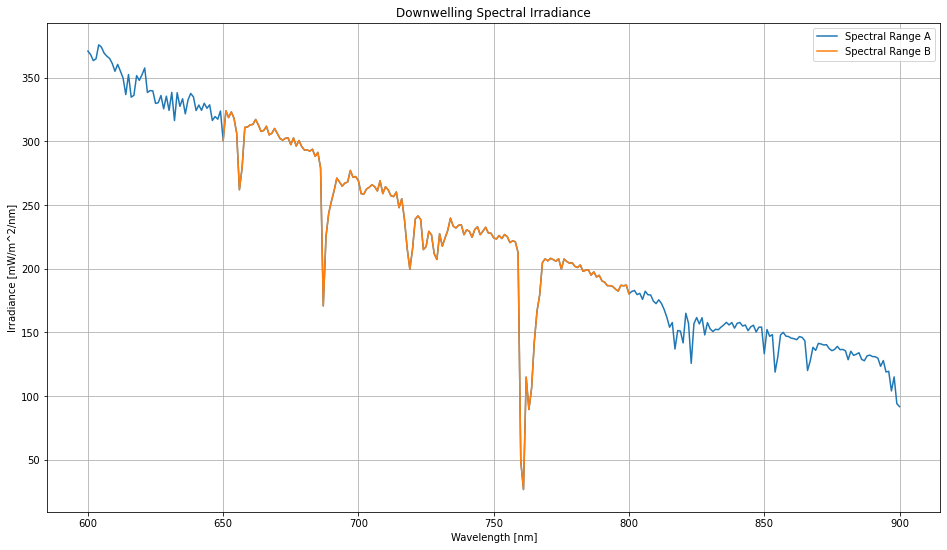
\includegraphics[width=0.6\textwidth]{./pic/libraddaskTemplate_13_0.png}
\end{center}


\begin{lstlisting}[style=tinysize]
# Check the quality of the Angstrom Law and King-Byrne formula fits
the_wv = np.arange(350.0, 950.0, 10.0)  # Pick a wavelength range
the_aot = librad.king_byrne_formula(the_wv, alpha_0, alpha_1, alpha_2)  # Calculate King-Byrne 
aot_ang = librad.angstrom_law(the_wv, alpha, beta)  # Calculate Angstrom Law
\end{lstlisting}


\begin{lstlisting}[style=tinysize]
# Plot Angstrom Law and King-Byrne fitted curves with MicroTOPS measurements
plt.figure(figsize=(16,9))
plt.plot(the_wv, the_aot, the_wv, aot_ang, aot_wv, aot, 'o')
plt.xlabel('Wavelength [nm]')
plt.ylabel('Aerosol Optical Thicknes')
plt.title('Aerosol Optical Thickness, Angstrom Law and King-Byrne Fit')
plt.legend(['King-Byrne', 'Angstrom', 'MicroTOPS'])
plt.grid()

\end{lstlisting}

\begin{center}
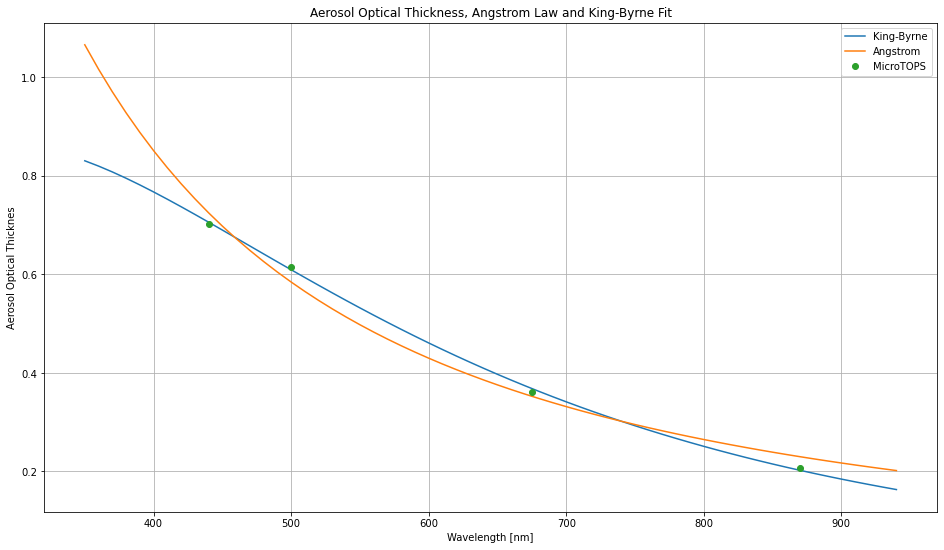
\includegraphics[width=0.6\textwidth]{./pic/libraddaskTemplate_15_0.png}
\end{center}


\section{Shutting down the Client}
\label{sec:ShuttingdowntheClient}

When the client is no longer required, shut it down.
\begin{lstlisting}[style=tinysize]
client.shutdown()
\end{lstlisting}
 % Serve use
% -*- TeX -*- -*- UK -*- -*- Soft -*-


\chapter{Conclusion}
\label{chap:Conclusion}

The \libraddask{} Python package provides a \libradtran{} server functionality to Python scripts and Jupyter notebooks.  The package is available on GitHub.

  % Conclusion
% \appendix
% \input{lic.tex}



\end{document}


